\documentclass[conference,onecolumn]{IEEEtran}
\usepackage{enumitem}
%\usepackage{cite}
\usepackage{graphicx}
\usepackage{float}
\usepackage{amsmath, nccmath, bm}
\usepackage{amssymb}
\graphicspath{{./images}}
\usepackage[backend=biber,style=ieee]{biblatex}
\addbibresource{sources.bib}

\title{XM Radio Reception with the PlutoSDR}

\author{
\IEEEauthorblockN{Owen Sowatzke}
\IEEEauthorblockA{\textit{Electrical Engineering Department} \\
\textit{University of Arizona}\\
Tucson, USA \\
osowatzke@arizona.edu}
\and
\IEEEauthorblockN{Glenn Alan Walker}
\IEEEauthorblockA{\textit{Electrical Engineering Department} \\
\textit{University of Arizona}\\
Tucson, USA \\
gaw@arizona.edu}}

\begin{document}
\maketitle

% Proposal
% XM radio leverages a combination of satellites and terrestrial repeaters to diversify its transmitted signal. The satellites transmit QSPK-modulated symbols, and the terrestrial repeaters leverage COFDM modulation \cite{5586866}. For our final project, we propose demodulating the signal from a single satellite and performing forward error correction (FEC). Our project will leverage the time, frequency, and frame synchronization methods covered in class. Additionally, it will extend the material covered in class to forward error correction. XM radio is a proprietary signal, and the technical details are documented only in patents such as \cite{a2008_us8260192b2, marko_2012_us8667344b2}. Major milestones for our project include: performing timing and frequency synchronization, extracting the master frame preamble (MFP) and frame synchronization preamble (FSP), and demodulating the signal from a single satellite. Additional stretch goals that will be addressed only if time permits include: demodulating the COFDM signals from terrestrial repeaters, combining the returns from multiple satellites and/or the terrestrial repeaters, and playing XM channel 1 audio (free preview channel). We believe that this project will reinforce what we learned in the course and provide invaluable experience performing FEC and OFDM demodulation.

\begin{abstract}
	In this project, we perform XM radio demodulation and forward error correction (FEC) in GNU radio using data captured with the Pluto SDR. GNU radio allows us to easily experiment with XM radio and rapidly prototype new receiver architectures. In our work, we concentrate on the time-domain multiplexed (TDM) satellite signals. To demodulate the signal, we leverage concepts learned in the class such as timing synchronization, carrier synchronization, and frame synchronization. As part of FEC, we also perform time deinterleaving, Virterbi decoding, and Reed Solomon Decoding.
\end{abstract}

\section{Introduction}

The final report covers the development and implementation of a software defined radio for the XM satellite radio service.  This report covers the basics of the XM radio signal from a physical layer standpoint.  The software included can capture and tune a single satellite signal to baseband bits.  The project covered all the labs in the ECE531 class with the exception of the radar lab.  The XM satellite radio system is proprietary and the project leverages the available U.S. patents and other publications to understand and decode the satellite signal.  These patents and publication are not specifications and could contain erronious information.  Care was taken to test each block to verify applicability to the published patents.

% In this project, we demodulate XM radio transmissions and perform forward error correction (FEC) with our Pluto SDR. XM radio uses a combination of satellites and terrestrial repeaters to diversify its transmitted signal. The satellites use QPSK modulation, and the terrestrial repeaters use coded orthogonal frequency domain multiplexing (COFDM). Our work focuses on the time-division multiplexed (TDM) signal from a single satellite. To demodulate this signal we leverage concepts from the course such as time synchronization, carrier synchronization, and frame synchronization. We also perform FEC, which was not covered in the course. With respect to FEC, we perform time deinterleaving, Virterbi decoding, and Reed Solomon Decoding. Because XM radio is a proprietary signal, it is documented only in patents such as \cite{a2008_us8260192b2, marko_2012_us8667344b2}. However, the patents leave out portions of the details, which require us to reverse-engineer portions of the system.

\section{Background}

% In this section, we provide background information on XM radio modulation. XM radio divides their content across two separate ensembles (Ensemble A and Ensemble B), which are illustrated in Figure \ref{fig::xm_satellite_config}. Each ensemble contains half of the XM radio channels and uses transmitter diversity to improve signal quality and prevent dropouts. The diversity scheme specifically uses QPSK-modulated signals from two separate satellites and a terrestrial COFDM-modulated signal.

XM is one of two satellite radio services that received FCC licenses in the U.S. to transmit digital radio services across the country.  XM received 12.5MHz of spectrum from 2332.5MHz to 2345MHz to operate in the U.S.  The XM system leverages a combination of satellites and terrestrial repeaters to diversify its transmitted signal. The satellites transmit QSPK-modulated symbols, and the terrestrial repeaters leverage COFDM modulation \cite{5586866}.  As illustrated in Figure \ref{fig::xm_satellite_config}, XM Radio divides their content across two separate ensembles (Ensemble A and Ensemble B).  When the service was launched in 2001, this service allocation allowed a receiver to tune to a single Ensemble reducing the hardware requirements.  Each ensemble uses transmitter diversity to improve signal quality and prevent dropouts. The diversity scheme specifically uses QPSK-modulated signals from two separate satellites and a terrestrial COFDM-modulated signal.  A total of 6 different digital transmissions are contained in the XM frequency band, 4 satellites signals and 2 terrestrial signals.

\iffalse
\begin{figure}[H]
	\centerline{\fbox{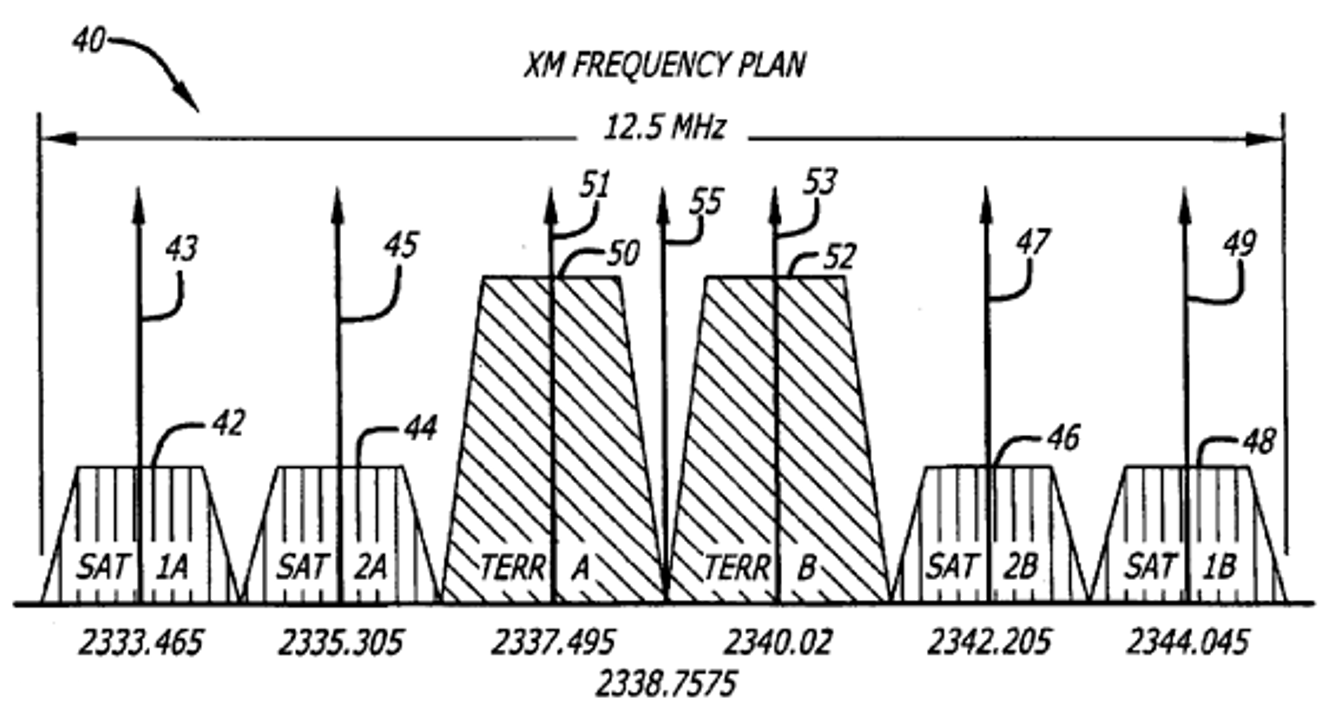
\includegraphics[width=0.5\textwidth]{xm_spectrum.png}}}
	\caption{XM Radio Spectrum \cite{a1999_us6724827b1}}
	\label{fig::xm_spectrum}
\end{figure}
\fi

\begin{figure}[H]
	\centerline{\fbox{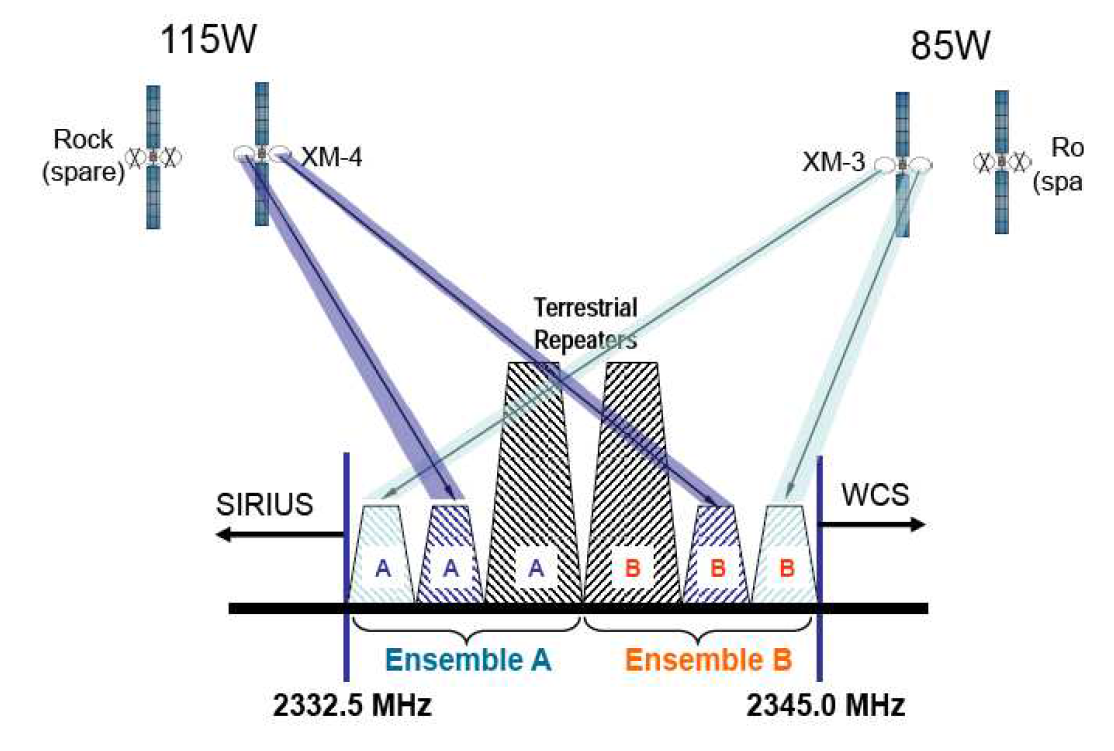
\includegraphics[width=0.5\textwidth]{xm_satellite_config.png}}}
	\caption{XM Radio Satellite Configuration \cite{5586866}}
	\label{fig::xm_satellite_config}
\end{figure}

	\noindent The center frequencies and bandwidths for each of the XM radio signals shown above have been derived from \cite{andreas_2010_us8594559b2} and are listed in Table \ref{table::center_freq_and_bw}:
\vspace{-12pt}
\begin{table}[H]
	\begin{center}
	\caption{XM Radio Center Frequencies and Bandwidths}
	\label{table::center_freq_and_bw}
	\begin{tabular}{| c | c | c |}
		\hline
		\textbf{Name} & $\mathbf{f_c}$ & \textbf{BW}\\
		\hline
		SAT1A & 2333.465 MHz & 1.886 MHz\\
		\hline
		SAT2A & 2335.305 MHz & 1.886 MHz\\
		\hline
		TERRA & 2337.490 MHz & 2.51 MHz \\
		\hline
		TERRB & 2340.020 MHz & 2.51 MHz \\
		\hline
		SAT1B & 2342.205 MHz & 1.886 MHz\\
		\hline
		SAT2B & 2344.045 MHz & 1.886 MHz\\
		\hline
	\end{tabular}
	\end{center}
\end{table}

% We concentrate specifically on the TDM receiver. An example of its architecture is displayed in Figure
% \ref{fig::tdm_receiver}.

% XM Radio divides their content across two separate ensembles (Ensemble A and Ensemble B), which are illustrated in Figure \ref{fig::xm_satellite_config}. Each ensemble uses transmitter diversity to improve signal quality and prevent dropouts. The diversity scheme specifically uses QPSK-modulated signals from two separate satellites and a terrestrial COFDM-modulated signal. We concentrate specifically on the TDM receiver. An example of its architecture is displayed in Figure \ref{fig::tdm_receiver}. 

\iffalse
\begin{figure}[H]
	\centerline{\fbox{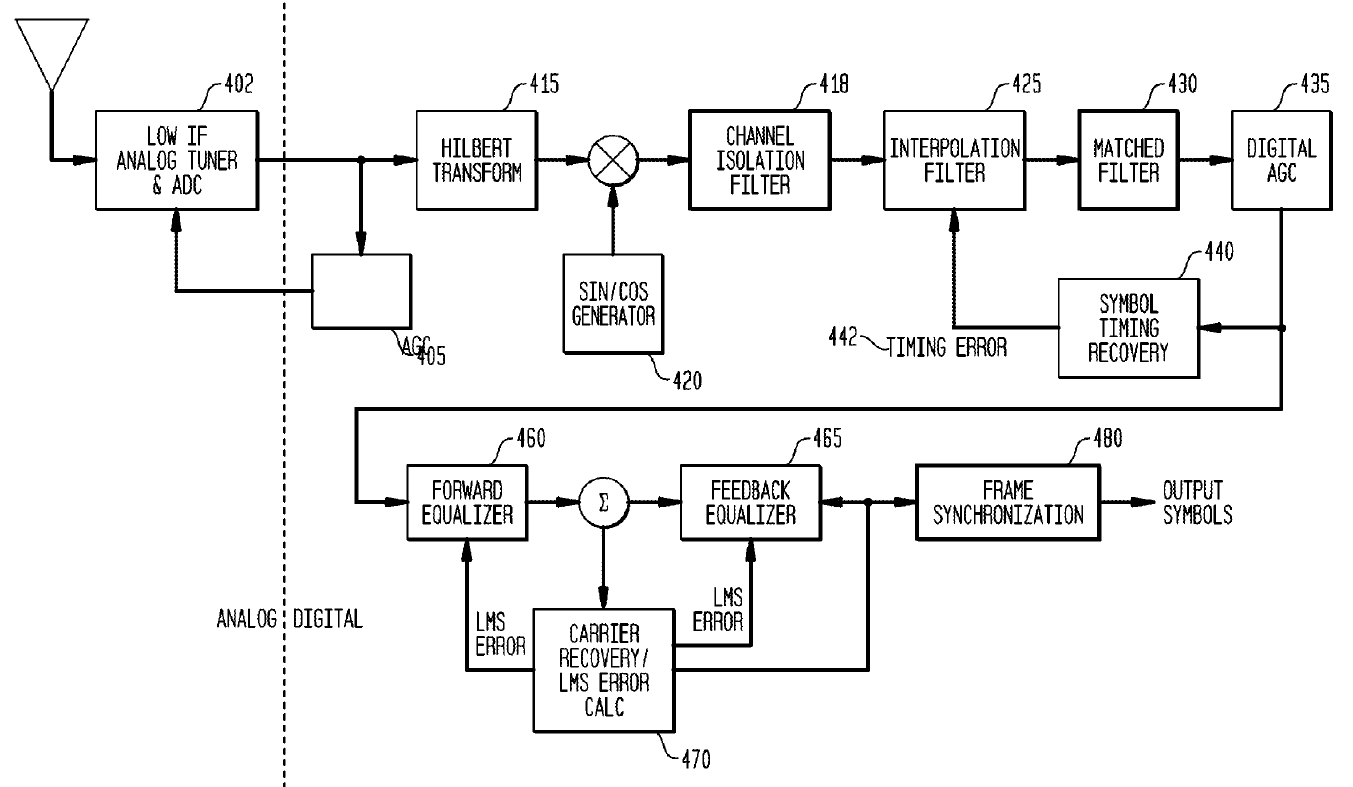
\includegraphics[width=0.5\textwidth]{tdm_receiver.png}}}
	\caption{TDM Receiver Architecture \cite{a2008_us8260192b2}}
	\label{fig::tdm_receiver}
\end{figure}
\fi

The report focuses on the satellite QPSK signals referred to as TDM (time division multiplex) signals. The TDM receiver architecture is illustrated in Figure \ref{fig::TDM_receiver2_8920000}. It is composed of a QPSK demodulator followed by a de-interleaver, Viterbi decoder, and Reed-Solomon decoder. An example QPSK demodulator is provided in the XM STA\_400a channel decoder chip specification and is attached for reference in Figure \ref{fig::TDM_receiver_STA400}. 

\begin{figure}[H]
	\centerline{\fbox{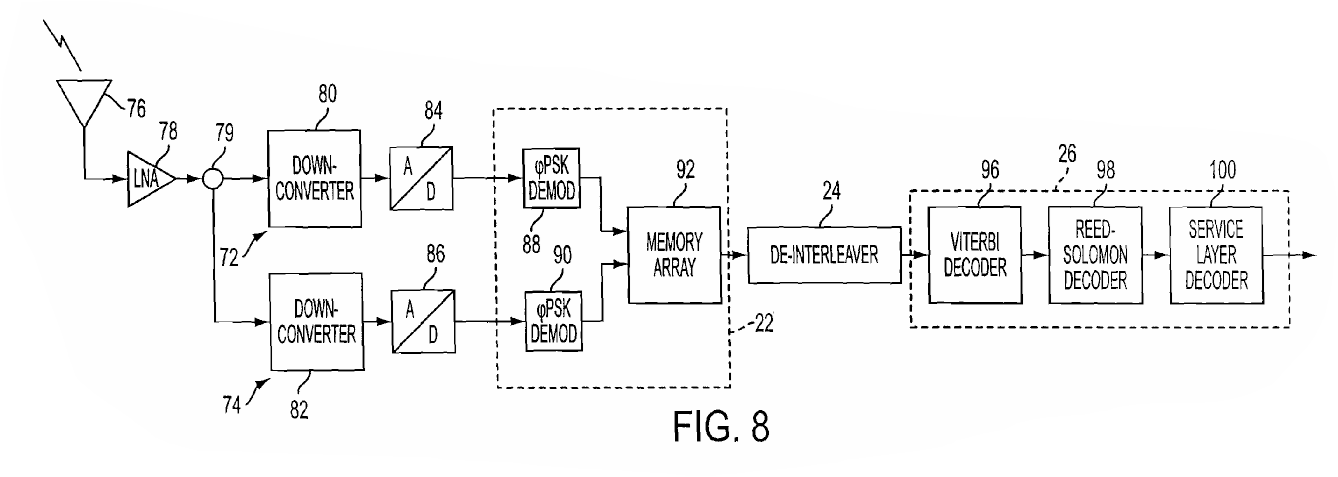
\includegraphics[width=0.5\textwidth]{TDM_receiver2_8920000.png}}}
	\caption{TDM Receiver Architecture \cite{marko_2012_us8667344b2}}
	\label{fig::TDM_receiver2_8920000}
\end{figure}

\begin{figure}[H]
	\centerline{\fbox{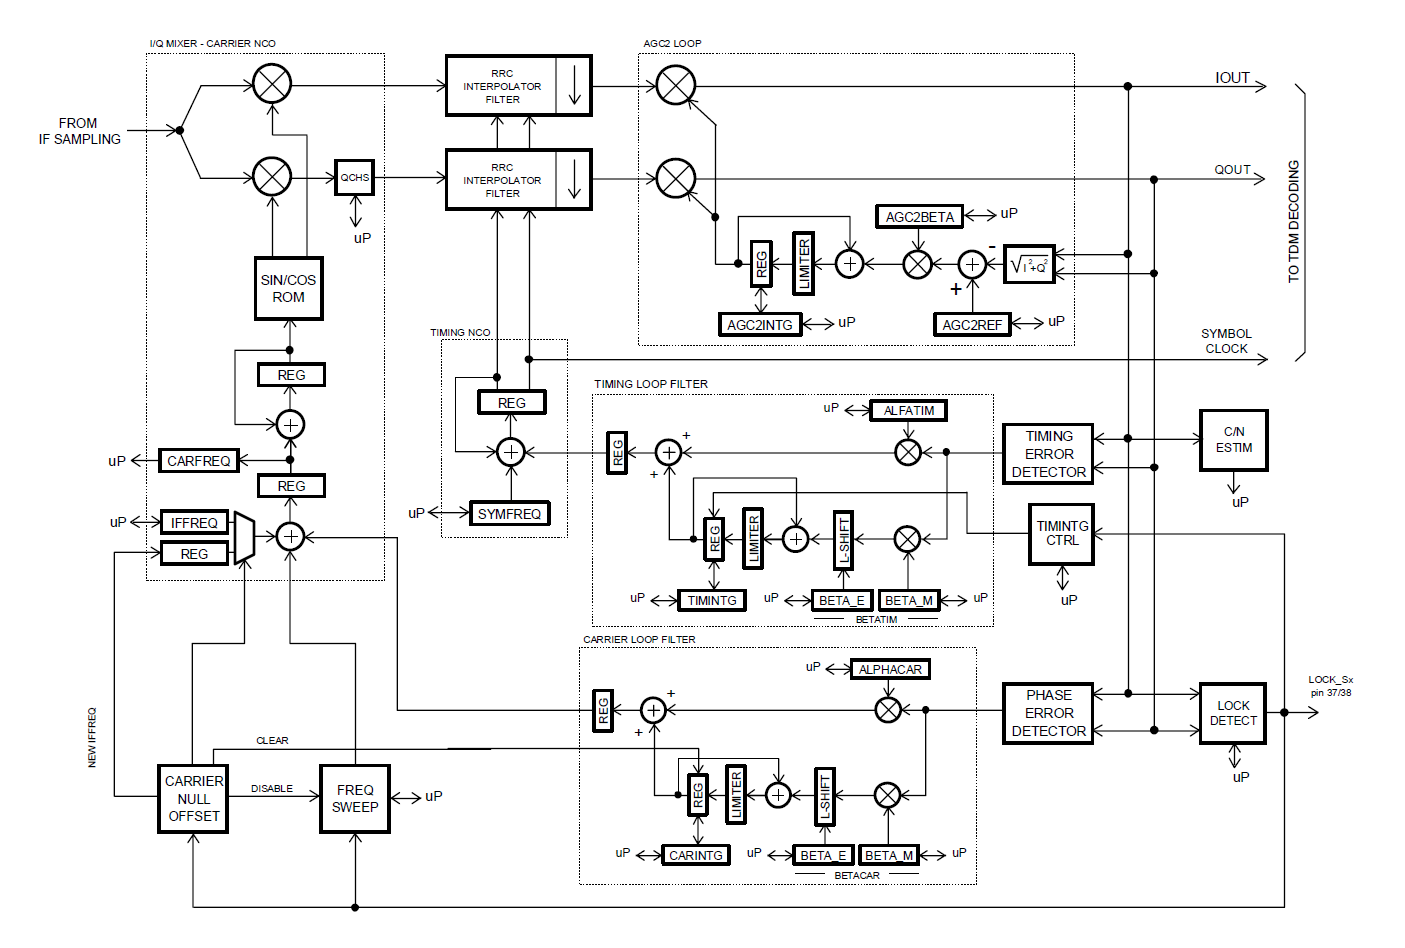
\includegraphics[width=0.5\textwidth]{STA_400_TDM_BLOCK_DIAGRAM.png}}}
	\caption{TDM QPSK Demodulator Details \cite{alldatasheetcom_2015_sta400a}}
	\label{fig::TDM_receiver_STA400}
\end{figure}

We can replace the structures from this datasheet with a more familiar architecture from class, which is shown in Figure \ref{fig::tdm_receiver_architecture}. In this updated figure, the carrier NCO block has been replaced with a coarse frequency correction block. The RRC interpolator filter has been replaced by the matched filter, and its interpolation has been moved into the timing synchronization block, which also includes the timing loop filter. Finally, the carrier loop filter has been replaced with a carrier recovery block. Additional background on each of these blocks is provided in the sections that follow. After describing the components of the QPSK demodulator, we also provide some background on each of the FEC blocks.

% We also perform frame synchronization, which is not included in the XM STA\_400a block diagram. 

% SHOULD WE INCLUDE AGC HERE
\begin{figure}[H]
	\centerline{\fbox{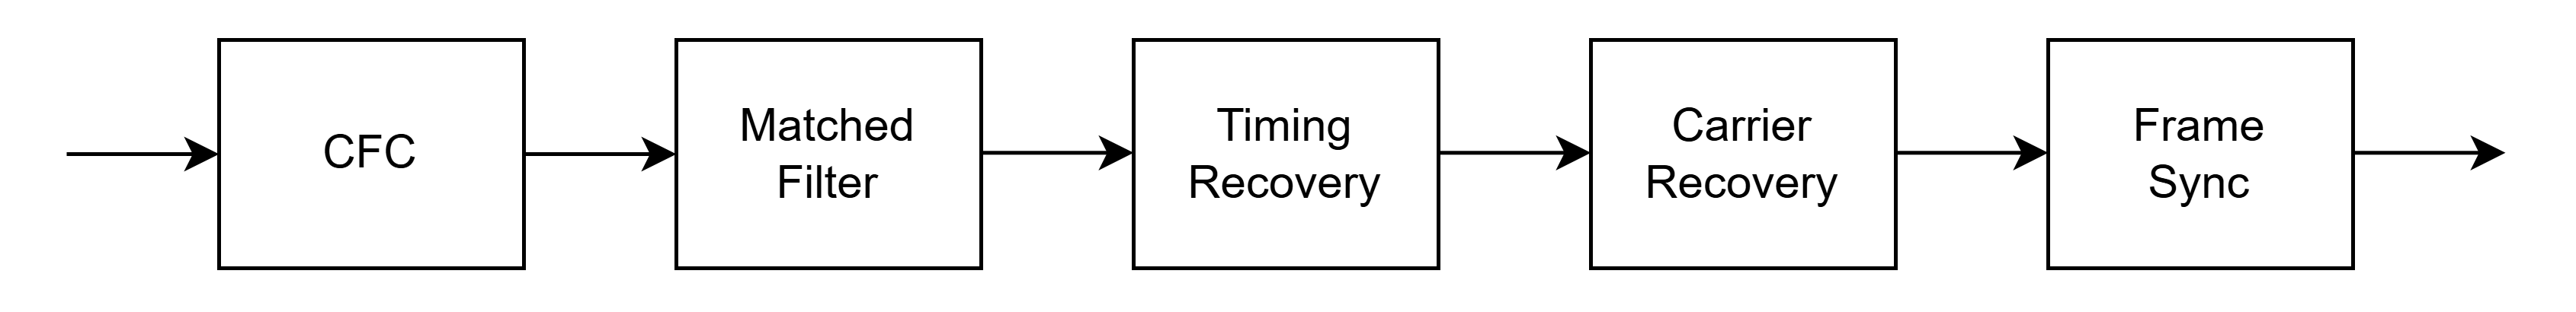
\includegraphics[width=0.8\textwidth]{tdm_receiver_architecture.png}}}
	\caption{TDM QPSK Demodulator Using Blocks from the Course}
	\label{fig::tdm_receiver_architecture}
\end{figure}

% In this report, we concentrate specifically on the SAT channels (TDM channels). A sample TDM receiver architecture is shown in Figure \ref{fig::tdm_receiver_architecture}. In this architecture, We start by performing coarse frequency compensation to remove large carrier offsets. Next, we pass the signal through a matched filter to maximize the SNR. Then, we perform timing recovery to ensure we are sampling the symbols in the ideal positions (midway between symbol transitions). We also perform carrier recovery to get rid of any residual phase or frequency offsets. Finally, we perform frame synchronization to form frames of data with the correct set of samples.

\subsection{Coarse Frequency Compensation}

Coarse frequency synchronization corrects for large carrier offsets, which can occur due to LO mismatches. We can write our base band signal with a frequency offset $f_o$ as follows:

\begin{equation}
	r(k) = s(k)e^{j(2{\pi}f_okT + \theta)}
\end{equation}

\noindent Additionally, for PSK modulated signals we know that the amplitude $s(k)$ is constant and the phase $\theta$ is defined as:

\begin{equation}
	\theta = \frac{2{\pi}n}{M},\quad n \in 0,1,...,M-1
\end{equation}

\noindent where $M$ is the constellation order. To determine the carrier frequency offset, we can raise our received data to the M-th power, which strips the modulation from our received data.

\begin{equation}
	r^M(k) = s^M(k)e^{j(2{\pi}f_okT + \theta)M} = s^M(k)e^{j2{\pi}Mf_okT}
\end{equation}

\noindent As previously stated, we can ignore the constant $s^M(k)$ term for PSK modulation. Then if we take an FFT of our data, we should be left with a sinc function centered about $Mf_oT$. In other words, we can solve for the coarse frequency offset as follows:

\begin{equation}
	\hat{f}_o = \frac{1}{MTK}\text{arg}\left|\sum_{k=0}^{K-1}{r^M(k)e^{-j2{\pi}kT/K}}\right|
	\label{eq::cfo_estimate}
\end{equation}

\noindent Then, to compensate for the coarse frequency offset, we can feed a negated copy of the coarse frequency offset ($-\hat{f}_o$) into an NCO and mix our signal with the result. Following the work of \cite{collins_2018_softwaredefined}, we specifically place our coarse frequency correction at the beginning of the chain to ensure that it operates on the largest possible bandwidth.
 
\subsection{Matched Filter}

The XM radio TDM signals use a square-root raised cosine (SRRC) filter for their matched filter with an excess bandwidth of 15\% \cite{a2008_us8260192b2}. The SRRC filter is a common type II Nyquist filter that is defined as follows:

\begin{equation}
	h(t) = \begin{cases}
		\dfrac{1}{\sqrt{T_s}}\left(1 - \beta + 4\dfrac{\beta}{\pi}\right), & t = 0 \\[12pt]
		\dfrac{\beta}{\sqrt{2T_s}}\left[\left(1 + \dfrac{2}{\pi}\right)\sin\left(\dfrac{\pi}{4\beta}\right)+ \left(1-\dfrac{2}{\pi}\right)\cos\left(\dfrac{\pi}{4\beta}\right)\right], & t = \pm\dfrac{T_s}{4\beta} \\[12pt]
		\dfrac{1}{\sqrt{T_s}}\dfrac{\sin\left[\pi\dfrac{t}{T_s}(1-\beta)\right]+4\beta\dfrac{t}{T_s}\cos\left[\pi\dfrac{t}{T_s}(1+\beta)\right]}{\pi\dfrac{t}{T_s}\left[1 - \left(4\beta\dfrac{t}{T_s}\right)^2\right]}, & \text{otherwise}
	\end{cases}
	\label{eq::srrc_filter}
\end{equation}

	Nyquist filters result in zero intersymbol interference (ISI), when they are correctly sampled at the midpoint of symbol transitions.  The Nyquist filter achieves zero ISI because its impulse response is zero at symbol intervals (i.e. $h(nT_s) = 0 \ \forall\ n \neq 0$). The sinc function is an example of type I Nyquist filter. Compared to the SRRC filter, it achieves a perfectly bandlimited frequency response. However, the impulse response is infinite time and decays with $1/t$, which does not converge in the presence of intersymbol errors. As a result, systems such as XM radio, use type II Nyquist filters, which have a finite impulse response that decays faster with time. However, compared to type I Nyquist filters, their frequency response is not perfectly bandlimited and will contain rolloff and excess bandwidth.
 
\subsection{Timing Synchronization}

	Nyquist filters, such as the SRRC filter, only result in zero ISI, when they are properly sampled at the midpoint of symbol transitions. Timing synchronization is used to compensate for imperfect sampling. The timing synchronization algorithm is illustrated in Figure \ref{fig::timing_synchronization}.

\begin{figure}[H]
	\centerline{\fbox{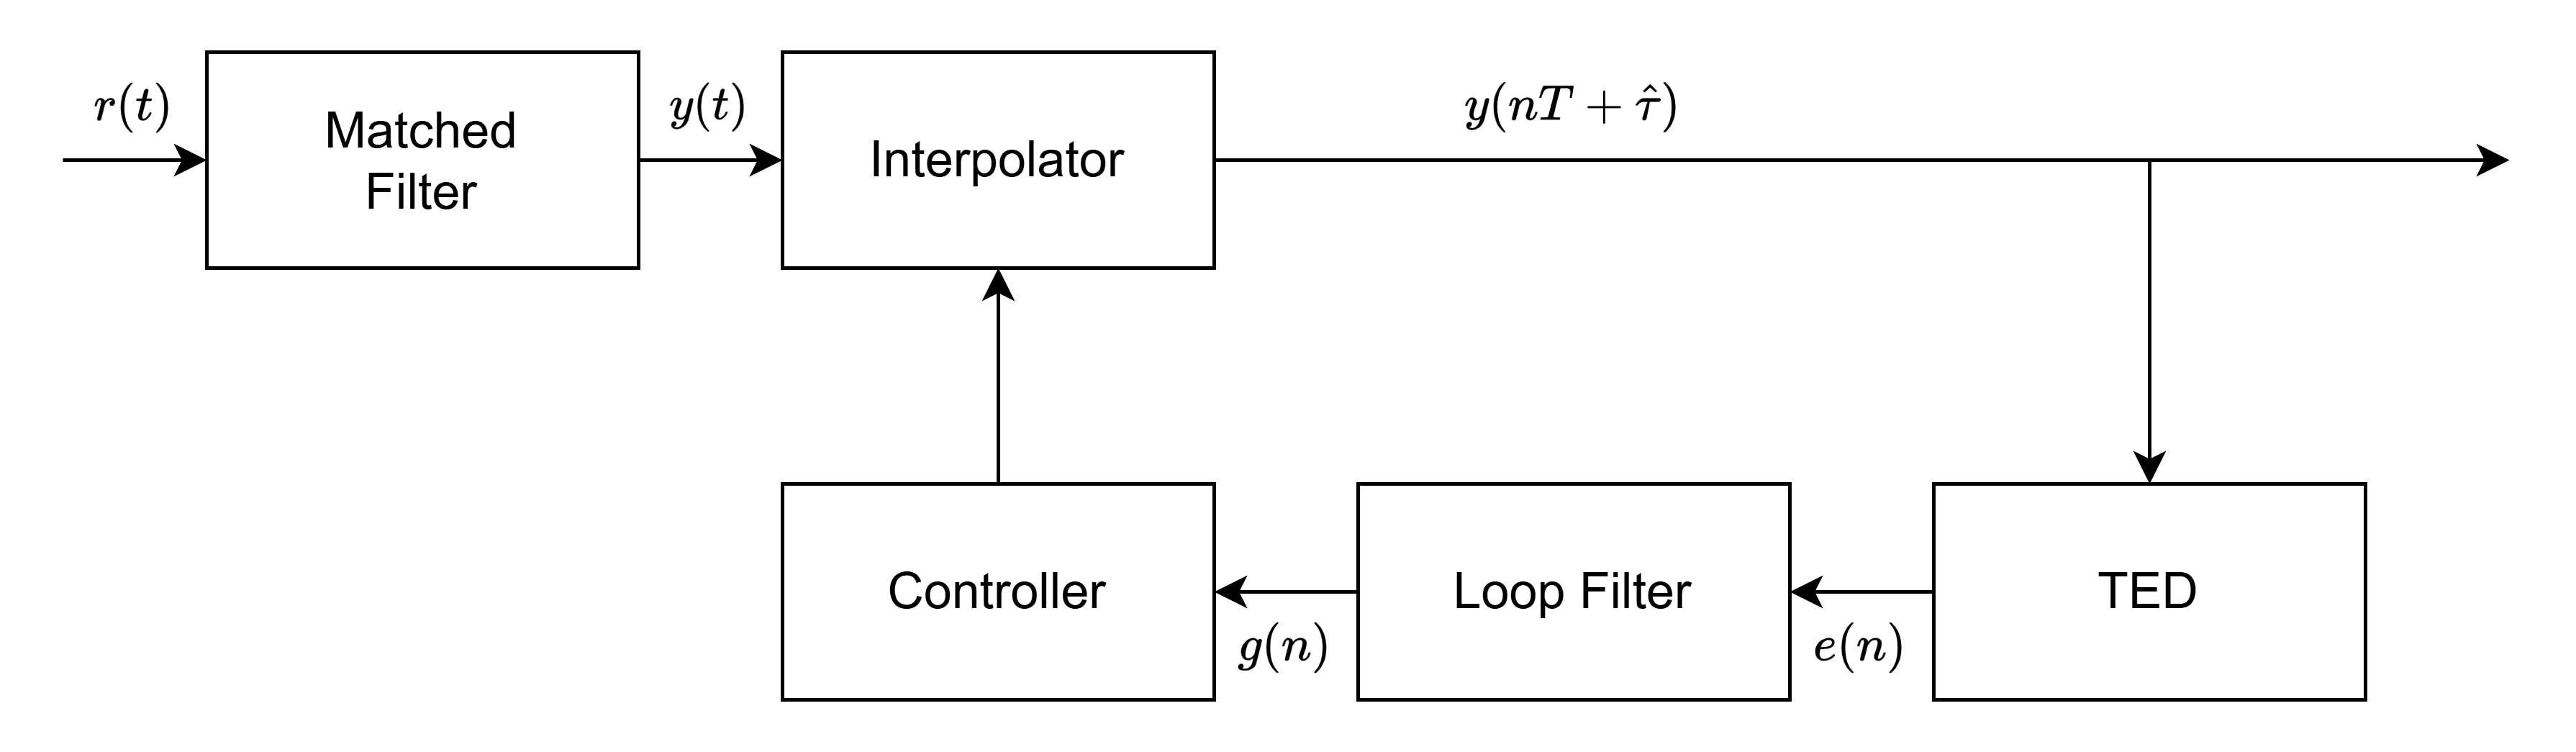
\includegraphics[width=0.6\textwidth]{timing_synchronization.png}}}
	\caption{Timing Synchronization Block Diagram}
	\label{fig::timing_synchronization}
\end{figure}

\subsubsection{Interpolator}

\noindent The interpolator applies a fractional delay to the input samples. For our interpolator, we specifically use a piecewise polynomial filter (PPF), which interpolates the input data as follows:

\begin{equation}
	x(kT_s + \mu(k)T_s) = \sum_{n=-2}^{1}{h(n)x((k-n)T_s)}
\end{equation}

\noindent where the filter taps $h(n)$ are given by

\begin{equation}
\begin{split}
	h = [&\alpha\mu(k)(\mu(k) - 1), \\
	&-\alpha\mu(k)^2 - (1-\alpha)\mu(k) + 1,\\
	&-\alpha\mu(k)^2 + (1+\alpha)\mu(k),\\
	&\alpha\mu(k)(\mu(k) - 1)]
\end{split}
\end{equation}

\subsubsection{Timing Error Detector}

\noindent The timing error detector (TED) measures the timing offset in the data. There are a few different methods for measuring these offsets. They include the zero crossing, Gardener, and  M\"{u}ller and Mueller methods. In the work that follows, we use the Gardener method because it is least sensitive to carrier phase offsets. The Gardener method defines the error signal $e(k)$ as follows:

\begin{equation}
\begin{split}
	e(k) =& \text{Re}(x((k-1/2)T_s+\tau))\left[\text{Re}(x((k-1)T_s + \tau)) - \text{Re}(x(kT_s + \tau))\right] + \\
	&\text{Im}(x((k-1/2)T_s+\tau))\left[\text{Im}(x((k-1)T_s+\tau)) -\text{Im}(x(kT_s+\tau))\right]
\end{split}
\end{equation}

\subsubsection{Loop Filter}

\noindent The timing error detector output is then fed into a loop filter which produces a stable signal for the controller. The loop filter uses a proportional integral (PI) filter, which is defined as follows:

\begin{equation}
	y(n) = G_1x(n) + G_2\sum_{k=0}^{n}{x(k)}
\end{equation}

\noindent In the above equations, $G_1$ and $G_2$ are constants and can be expressed in terms of the normalized loop bandwidth ($B_{\text{Loop}}$), the damping factor ($\zeta$), the samples per symbol ($N$), and the detector gain ($G_D$). They are specifically defined as follows:

\begin{align}
	G_1 = \frac{-4\zeta\theta}{G_DN\Delta} && G_2 = \frac{-4\theta^2}{G_DN\Delta}
	\label{eq::loop_filter}
\end{align}

\noindent where $\theta$ and $\Delta$ are given by:
\begin{align}
	\theta = \frac{B_{\text{Loop}}}{M(\zeta + 0.25/\zeta)} && \Delta = 1 + 2\zeta\theta + \theta^2
\end{align}

\subsubsection{Interpolation Controller}

The interpolation controller computes a fractional delay and a strobe which indicates when the delay should be applied. The strobes occur on average once per symbol. The counter decrement value can be computed with the loop filter output $v(n)$ as follows:

\begin{equation}
	W(n) = v(n) + \frac{1}{N}
\end{equation}

\noindent Using the decrement value, the counter is updated as follows:

\begin{equation}
	c(n + 1) = (c(n) - W(n))\ \text{mod}\ 1
\end{equation}

\noindent Strobes occur whenever the counter wraps.

\begin{equation}
	\text{Strobe} = \begin{cases}
		\text{True}, & \text{if}\ c(n) < W(n)\\
		\text{False}, & \text{otherwise}
	\end{cases}
\end{equation}

\noindent Finally, on each strobe, we update the factional delay parameter as follows:

\begin{equation}
	\mu(k) = \frac{c(n)}{W(n)}
\end{equation}

\subsection{Carrier Recovery}

In this section, we describe the carrier recovery block. The carrier recovery block is responsible for fine frequency synchronization as opposed to the coarse frequency compensation block at the front of the chain. An overview of the fine frequency synchronization is displayed in Figure \ref{fig::carrier_synchronization}.

\begin{figure}[H]
	\centerline{\fbox{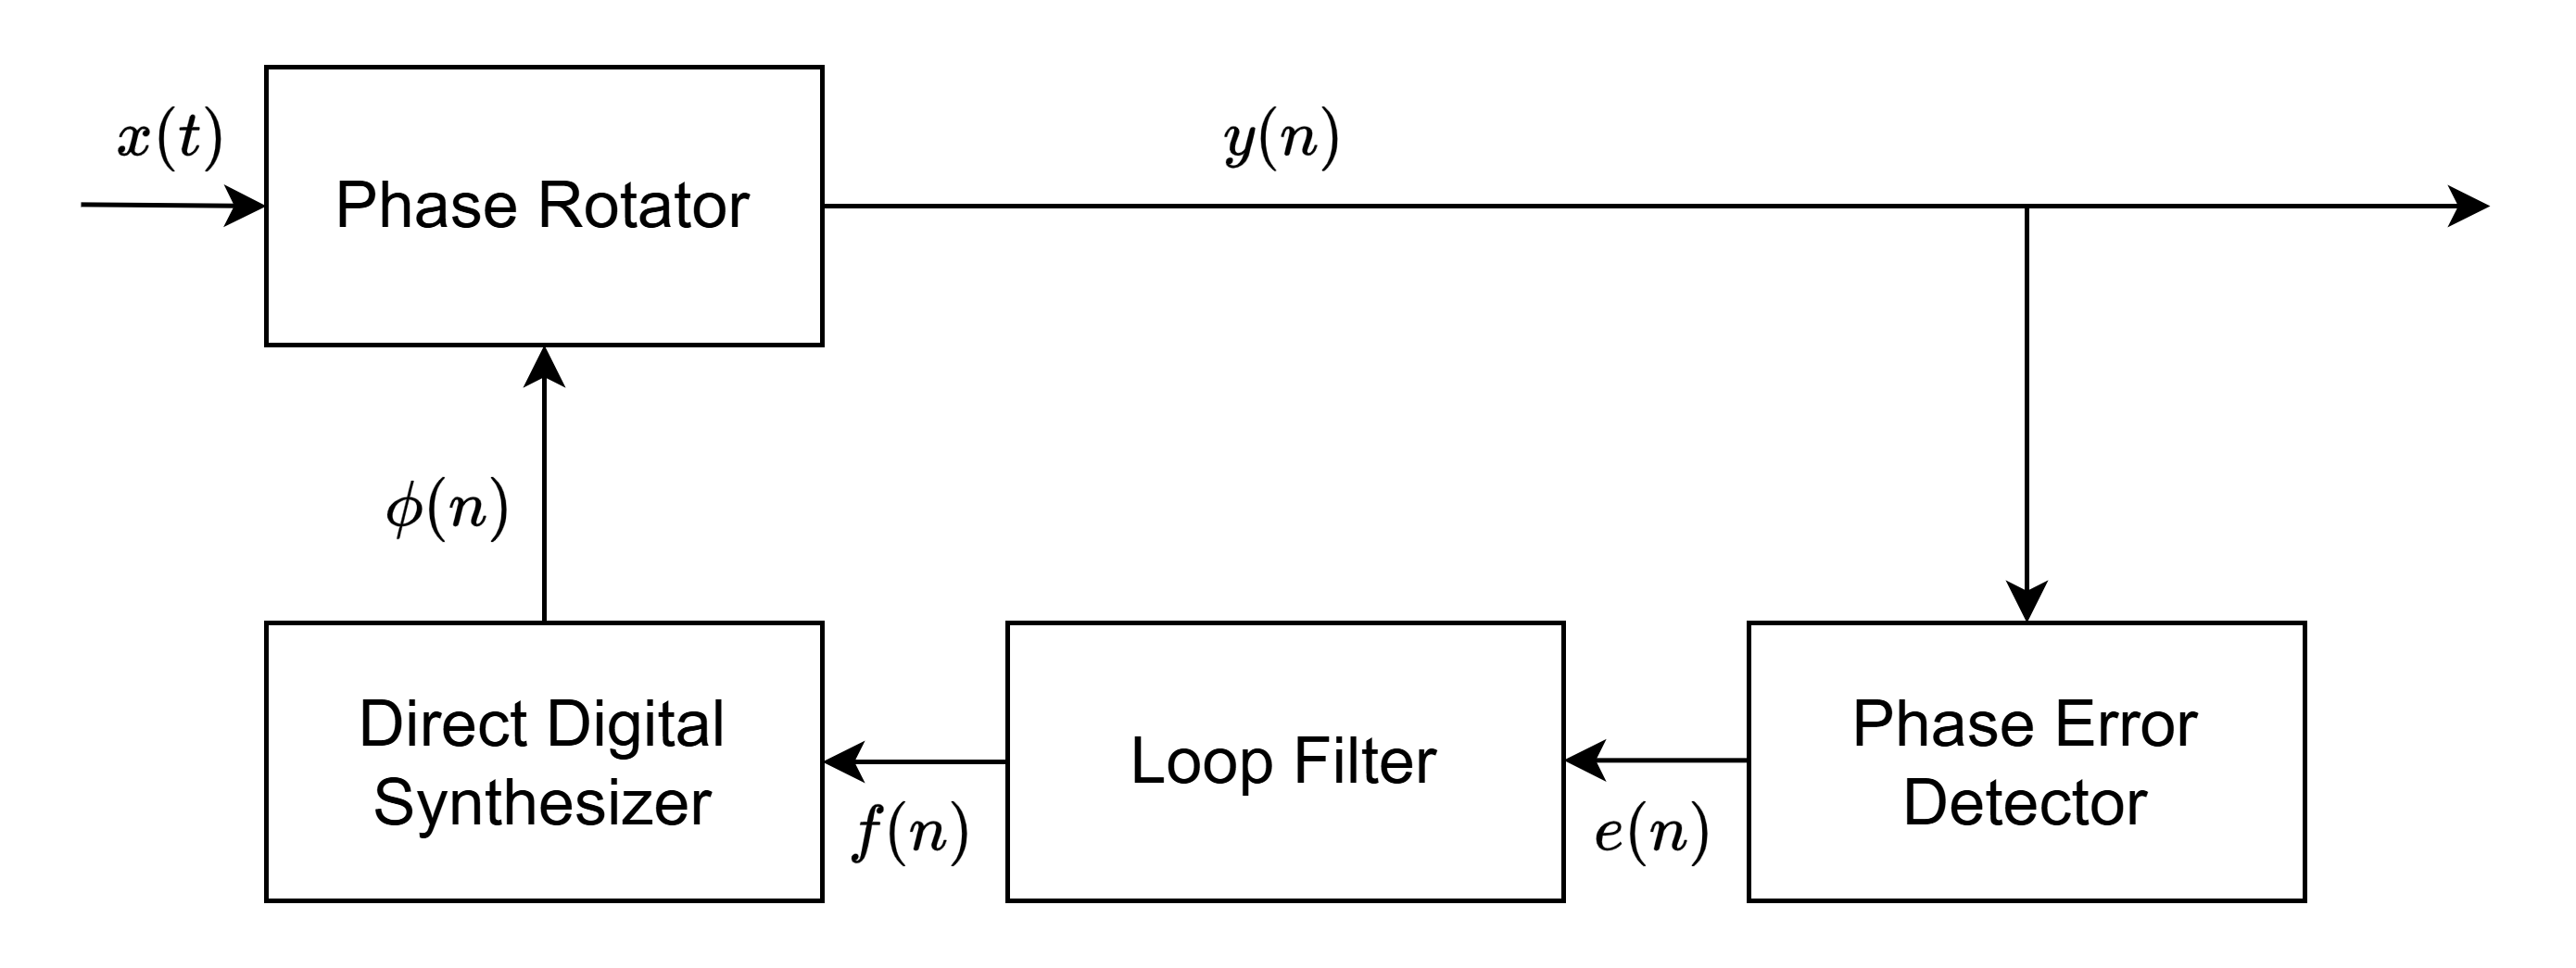
\includegraphics[width=0.5\textwidth]{carrier_synchronization.png}}}
	\caption{Fine Frequency Synchronization}
	\label{fig::carrier_synchronization}
\end{figure}

The carrier synchronization architecture is very similar to the the timing synchronization architecture. It uses a phase error detector (PED) to detect phase offsets in the received data. Then, it stabilizes the error signal in the loop filter, which feeds a direct digital synthesizer (DDS). The DDS generates a correction signal which is applied in the phase rotator.

\subsubsection{Phase Error Detector}

The phase error detector is chosen based on the modulation scheme. The TDM receiver uses QPSK modulation. Therefore, we compute the error signal ($e(k)$) as follows:

\begin{equation}
	e(k) = \text{sign}(\text{Re}(y(k))) \times \text{Im}(y(k)) - \text{sign}(\text{Im}(y(k))) \times \text{Re}(y(k))
\end{equation}

\noindent In the above equation, the error signal is zero when, $\text{Re}(y(k)) = \pm\text{Im}(y(k))$. By minimizing the error signal, fine frequency synchronization will force the received data to the nearest QPSK constellation point.

\subsubsection{Loop Filter}

The loop filter is responsible for stabilizing the error signal. It uses the same proportional-plus integrator (PI) filter that was presented in Equation \ref{eq::loop_filter} with updated values for $G_1$ and $G_2$. The updated constants are defined in terms of the damping factor ($\zeta$), the loop bandwidth $B_{\text{Loop}}$, and the modulation order ($M$).

\begin{align}
	G_1 = \frac{4\zeta\theta/\Delta}{M} && G_2 = \frac{(4/M)\theta^2/\Delta}{M}
\end{align}

\noindent where $\theta$ and $\Delta$ are defined as follows:

\begin{align}
	\theta = \frac{B_{\text{Loop}}}{M(\zeta + 0.25/\zeta)} && \Delta = 1 + 2\zeta\theta + \theta^2
\end{align}

\noindent The selection of $\zeta$ affects the responsive and stability of the PLL:

\begin{equation}
\zeta = \begin{cases}
< 1, & \text{Underdamped}\\
= 1, & \text{Critically Damped}\\
> 1, & \text{Overdamped}
\end{cases}
\end{equation}

\noindent $B_\text{Loop}$ is then chosen to achieve a maximum frequency pull-in range, $\Delta_{f,\text{pull}}$, and a maximum frequency lock delay, $t_{\Delta,\text{Max}}$, which are defined in \cite{collins_2018_softwaredefined} as follows:

\begin{equation}
	\label{eq::max_freq_correct}
	\Delta_{f,\text{pull}} \sim 2\pi\sqrt{2}\zeta{B_\text{Loop}}\end{equation}

\begin{equation}
	t_{\Delta,\text{Max}} \sim \frac{32\zeta^2}{B_\text{Loop}}\end{equation}

\subsubsection{Direct Digital Synthesizer}

The direct digital synthesizer creates a tone using the phase output by the loop filter. It specifically performs phase accumulation to determine the instantaneous phase of the correction signal. The transfer function for the DDS is specifically given by:

\begin{equation}
	D(z) = G_3\frac{z^{-1}}{1 - z^{-1}}
\end{equation}

\noindent where $G_3 = -1$ to remove the phase offset from the received signal. Note that our accumulator also includes an additional cycle of delay to simplify the implementation.

\subsubsection{Phase Rotator}

The phase rotator creates a tone from the phase output by the DDS using a lookup table (LUT). The received signal is then multiplied with this tone to remove the phase and frequency offsets.

\subsection{Frame Synchronization}

XM radio divides its transmitted data into frames. These frames include two different preambles: the MFP (master frame preamble) and the FSP (fast synchronization preamble). The FSP marks the start of the data portion and corrects for ambiguities, while the MFP is used to align the signal from each satellite \cite{a2008_us8260192b2}. Both preambles and their relative timing are illustrated in Figure \ref{fig::tdm_frame_format}.

\begin{figure}[H]
	\centerline{\fbox{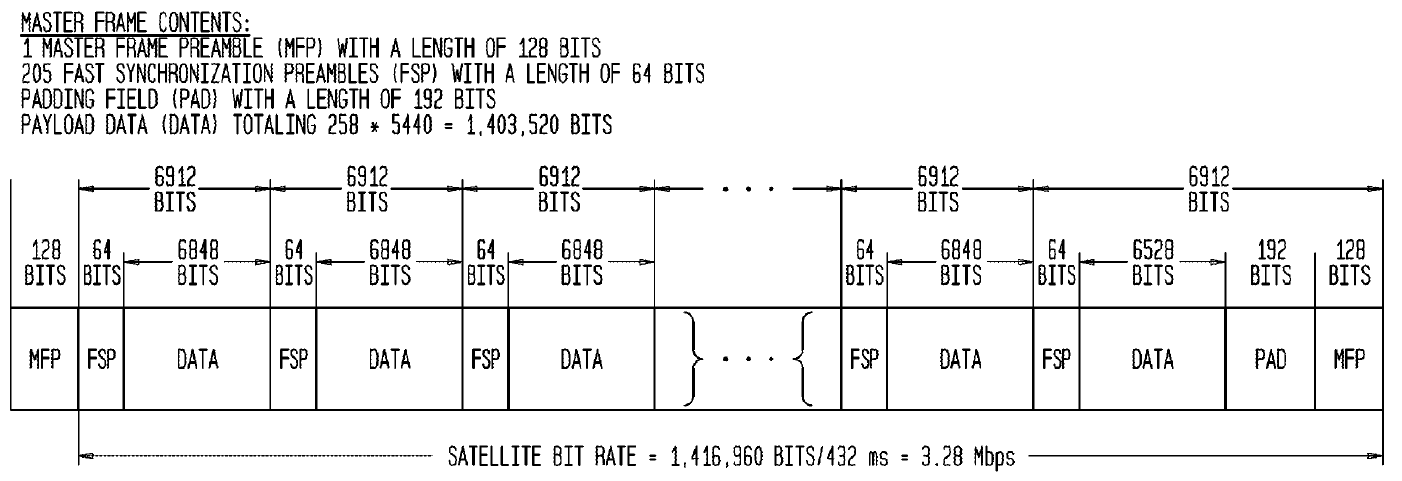
\includegraphics[width=0.8\textwidth]{tdm_frame_format.png}}}
	\caption{TDM Frame Format \cite{a2008_us8260192b2}}
	\label{fig::tdm_frame_format}
\end{figure}

\noindent We can detect both of these preambles by cross-correlating our received data with each preamble. The cross-correlation is specifically given by:

\begin{equation}
	C_{xy}(k) = \sum_m{x^*(m)y_n(m+k)}
\end{equation}

\noindent The peak of the cross-correlation output should correspond to the delay of the preamble. MATLAB's \text{xcorr} function outputs the correlation for positive and negative values of $m$. Therefore, the delay ($\hat{p}$) is given by

\begin{equation}
	\hat{p} =  \underset{k}{\text{argmax}}\ C_{xy}(k) - L_r
\end{equation}

\noindent where $L_r$ is the length of the longest input sequence. We can also use MATLAB's \texttt{filter} command to more efficiently compute the cross-correlation for short input sequences. The \texttt{filter} command performs convolution, which is given by the following formula:

\begin{equation}
	z(k) = \sum_{m}{y_n(m)h(k - m)}
\end{equation}

\noindent To use the \texttt{filter} command for cross-correlation, we need the filter $h(k)$ to be $x^*(-k)$. The \texttt{filter} command peaks when the last sample of the preamble is aligned with the filter. Therefore, we can define the delay as follows:

\begin{equation}
	\hat{p} = \underset{k}{\text{argmax}}\ z(k) - L_p
\end{equation}

\noindent where $L_p$ is the length of the preamble. Depending on what libraries are used for correlation, these delays may vary slightly. To simplify our thresholding, we can also normalize the signal so it has unit average power over the correlation window.

\subsection{Time Interleaver}

XM requires time diversity in its service to ensure minimum dropouts for paying customers.  To accomplish this, XM uses a convolutional time interleaver to spread the transmitted bits over a wide period time (specifically 4.69 seconds).  Time diversity allows the receiver to recover the transmitted signal with large signal blockage time. 

In the XM radio MFP structure, the data is partitioned into PRC ``prime rate channels'' which consist of 258 PRC's grouped as 5440 transmitted bits each as seen in Figure \ref{fig::tdm_frame_format}.  These 5440 bits PRCs are the results of the FEC encoding, which uses a RS(255,223) block code (Reed Solomon) followed by a convolutional encoding at rate 3/8.  A RS (255,223) encoder produces 2040 transmitted bits and the rate 3/8 convolution encoding increases the transmitted bits to 5440.  Each satellite transmits 1/2 the bits or 2720 bits. 

% Details of the FEC encoding will follow in FEC section (what FEC section?)

Each PRC of 5440 bits per satellite is the result of 2 RS codewords.  As can be seen in Figure \ref{fig::time_interleaver} obtained from \cite{marko_2012_us8667344b2}, XM radio uses a separate convolutional time interleaver on each PRC.

\begin{figure}[H]
	\centerline{\fbox{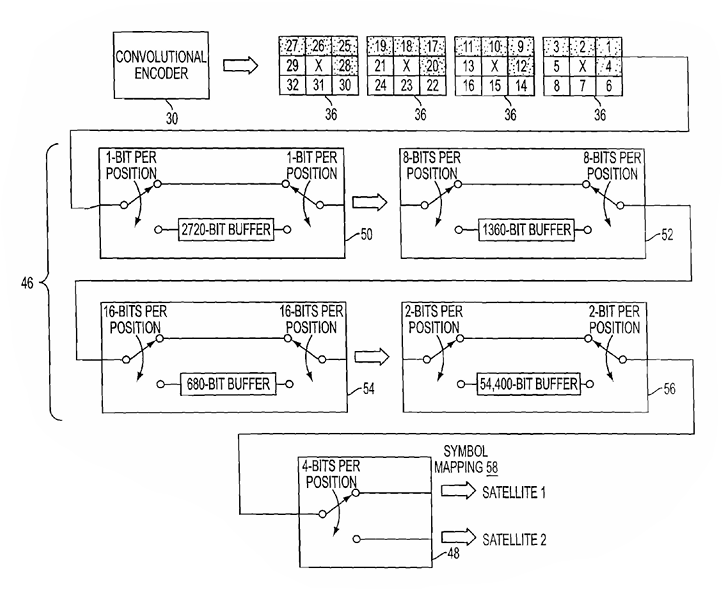
\includegraphics[width=0.8\textwidth]{XM_TIME_INTERLEAVER_DETAILS_no_label.png}}}
	\caption{XM Time Interleaver \cite{marko_2012_us8667344b2}}
	\label{fig::time_interleaver}
\end{figure}

% Explain how we can process the satellite independently

Figure \ref{fig::time_interleaver} shows the time interleaver from the transmitter's point of view.  The receiver follows in reverse. As can be seen, each satellite can be processed independently or combined in a receiver through this time interleaver mechanism.  For our tests, we used a single satellite (sat2) as the source and inserted zeros for the other satellite (sat1). Block 36 highlights the punctured bits (marked by an X), satellite 1 bits (1-4), and satellite 2 bits (5-8).  As can be seen in Figure \ref{fig::time_interleaver}, when one uses 5440 bits per MFP (0.432 ms) and calculates the maximum delay through the 4 buffers, the result is an interleaver delay of 4.698 seconds described in the XM chipset STA400a section 1.4 TDM DECODING \cite{alldatasheetcom_2015_sta400a}.

\subsection{Convolutional Decoder}

A convolutional encoder/decoder uses a concept similar to FIR/IIR filters, where the information bits are spead over time using GF(2).  These codes have been around since the 1950's.  These codes use registers to keep track of the state of the system.  They can use both recursive and non-recursive feedback polynomials to spread the information bits across time.  Non-recursive convolutional codes are commonly decoded with the Viterbi algorithm and recursive polynomials are commonly used in Turbo codes.

XM uses a non-recursive convolutional encoder/decoder as part of the concatenated coding.  Concatenated codes typically use an inner convolutional code with an outer block code.  For the XM sytem, they employ a complementary convolutional encoder.  This is a way to split the transmitted information across the two satellites as well as the terrestrial signal.  Figure \ref{fig::Viterbi} shows details of the convolution encoder described in XM patent \cite{marko_2012_us8667344b2}.  This encoder takes in 3 information bits and create 9 transmitted bits.  The bits labeled ``A'', ``B'', ``C'' and ``D'' are sent to satellite 1 and bits ``F'', ``G'', ``H'' and ``J'' are sent to satellite 2.  The terrestrial signal uses the same bits as satellite 2 with the addition of bit ``E''.

\begin{figure}[H]
	\centerline{\fbox{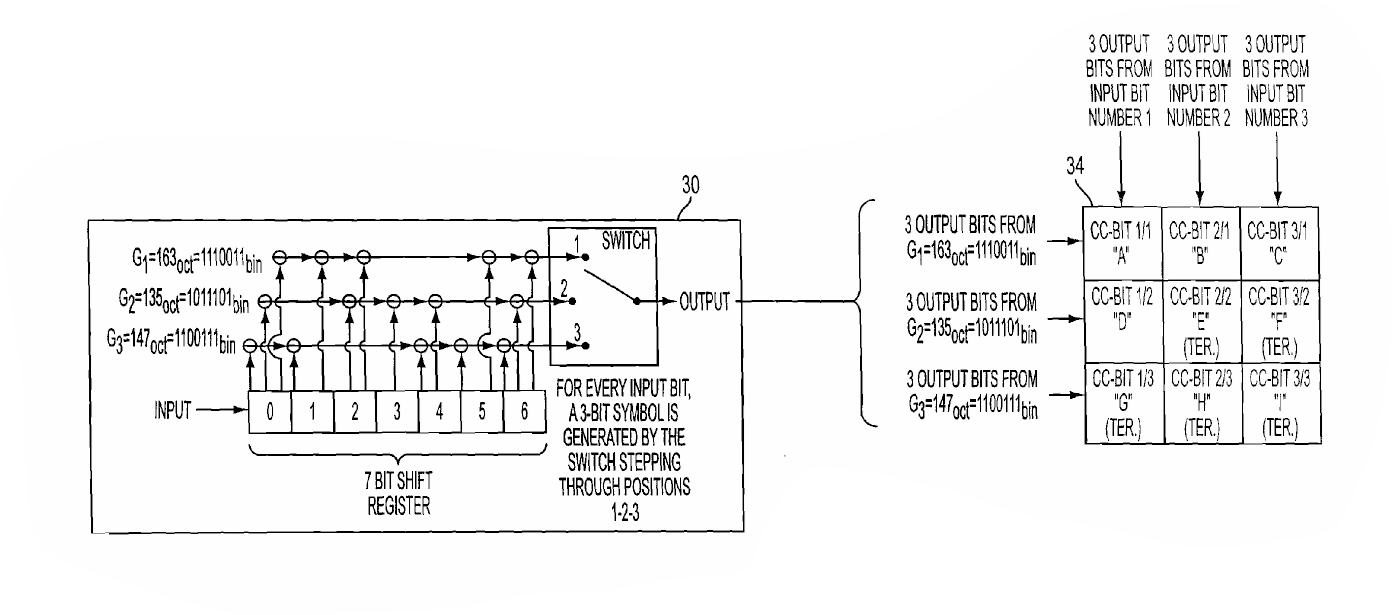
\includegraphics[width=0.8\textwidth]{Viterbi_encoder.png}}}
	\caption{XM Convolutional Encoder \cite{marko_2012_us8667344b2}}
	\label{fig::Viterbi}
\end{figure}

\subsection{Reed Solomon Decoder}

Reed Solomon codes are block-based error correction codes. For XM radio, they define their Reed Solomon code over $\text{GF}\left(2^8\right)$. They specifically use a (255,223) Reed Solomon code. In other words they encode 223 data symbols in 255 symbols, where the extra 32 symbols serve as parity. This allows the XM radio to correct up to 16 symbol errors \cite{a2008_us8260192b2}. Because the Reed Solomon code operates on bytes, it is also very good at correcting bursts of errors, which can occur when there is fading.

\section{Procedure}

In this section, we provide the procedure for our project. The procedural flow through each of the major blocks in our system is illustrated in Figure \ref{fig::xm_radio_processing}. Note that the most of the stages have been broken up with files. These files allow us to incrementally develop our algorithms and generate repeatable results in each stage of processing. Once the system is complete, these files can be removed and all the logic can be consolidated into a single GNU radio flowchart, which leverages existing blocks and custom blocks.

\begin{figure}[H]
	\centerline{\fbox{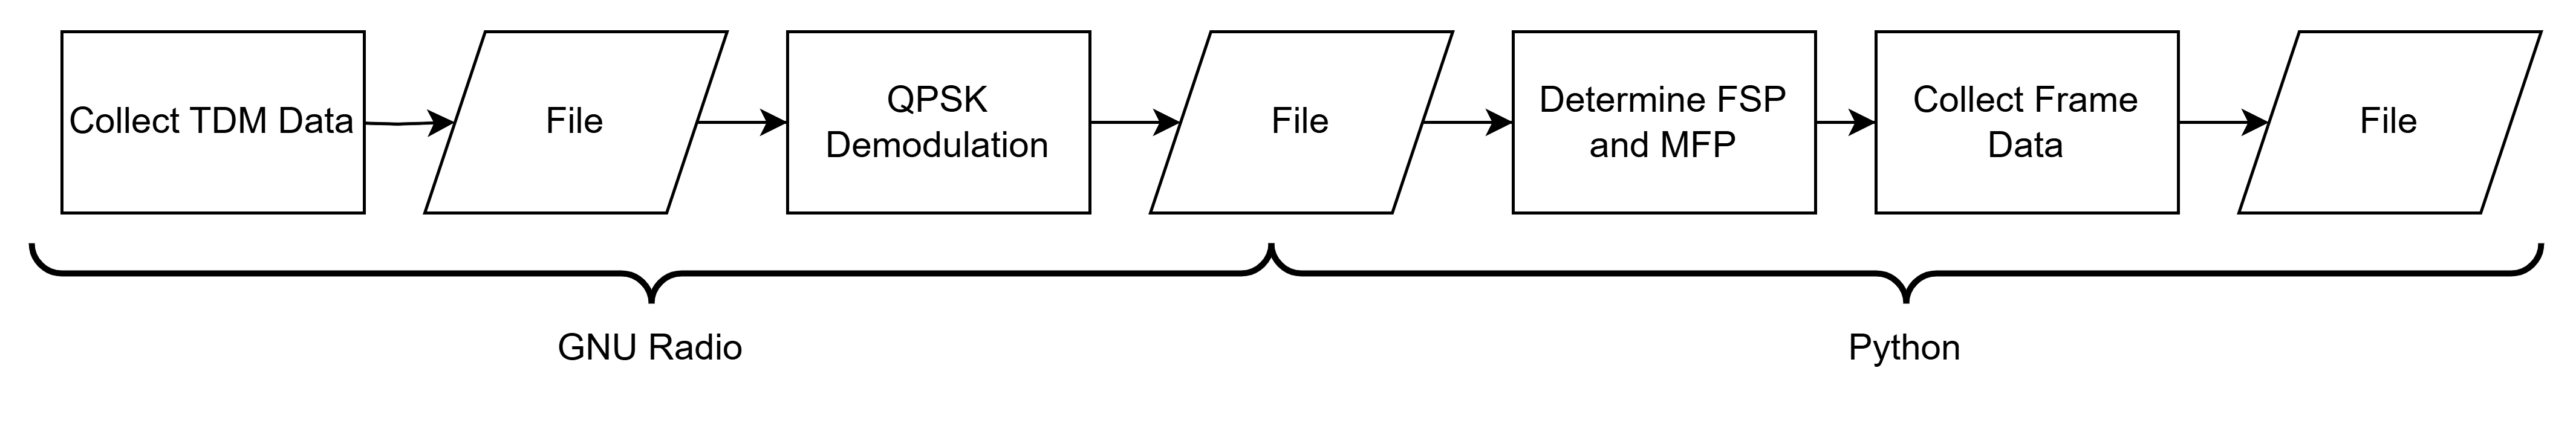
\includegraphics[width=0.95\textwidth]{xm_radio_processing.png}}}
	\caption{XM Radio Procedural Flow for Project}
	\label{fig::xm_radio_processing}
\end{figure}

\subsection{TDM Signal Collection}

A GNU radio companion setup was created (see Figure \ref{fig::gnu_collect}) to collect the satellite signal at 2335.305MHz.  An active antenna is useful to maximize the signal to noise ratio for satellite to earth transmission.  XM radio active antennas typically have around 25dB of gain with an approximately 1dB  noise figure.  The PlutoSDR has a relatively high noise figure on the receive port and attaching an active antenna in front reduces the overall noise into the receiver.  To enable the collection of the best signal possible, the setup in Figure \ref{fig::gnu_hardware} was used.  To get power to the antenna, a RF bias-T was used.  After confirming that the signal was sufficiently strong, a recording of about 20 seconds was made.
\begin{figure}[H]
	\centerline{\fbox{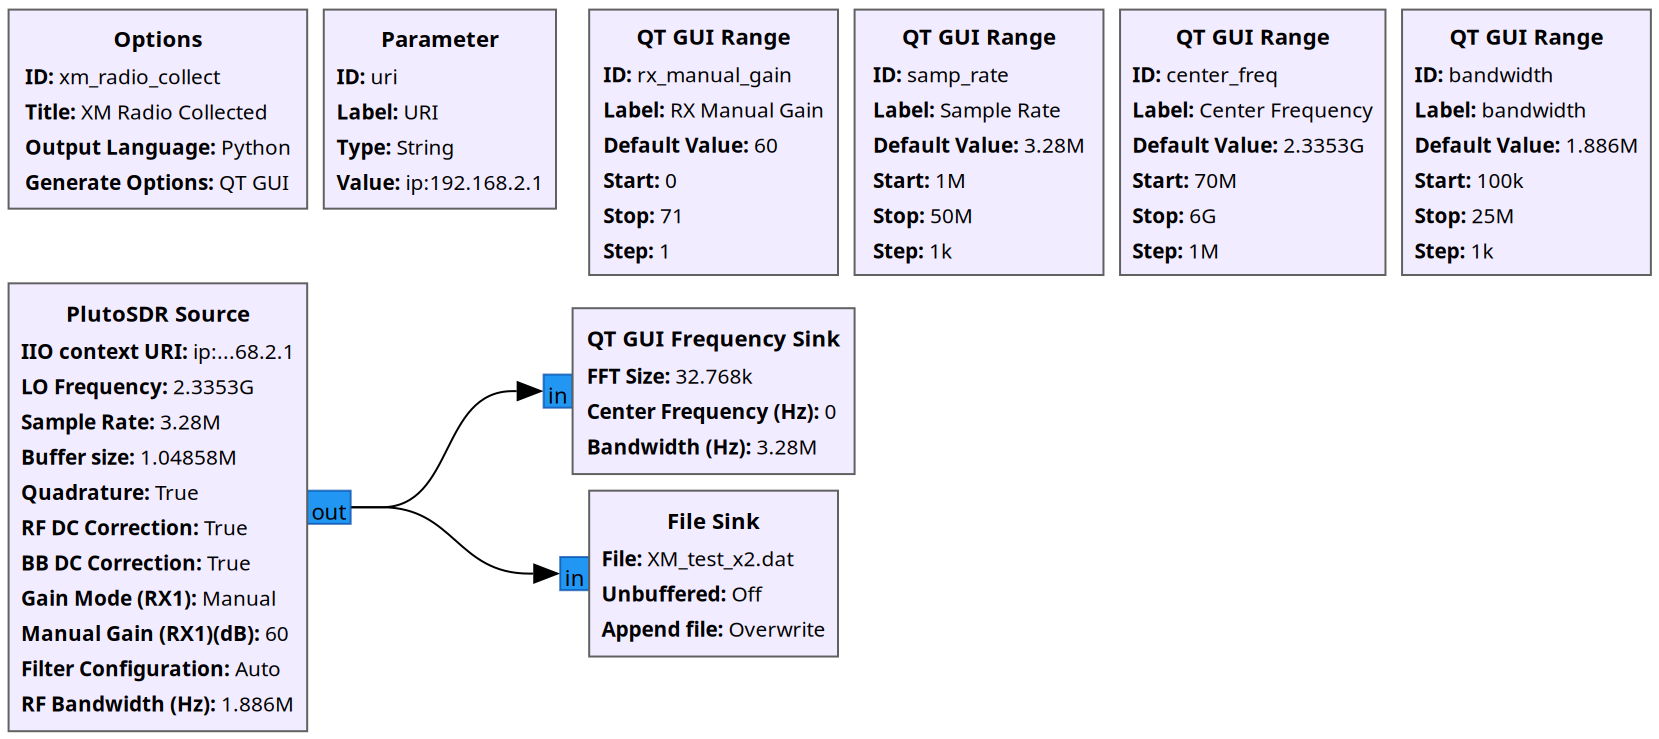
\includegraphics[width=0.5\textwidth]{XM_collect_grc.png}}}
	\caption{GNU Radio Flowchart for Signal Collection}
	\label{fig::gnu_collect}
\end{figure}
\begin{figure}[H]
	\centerline{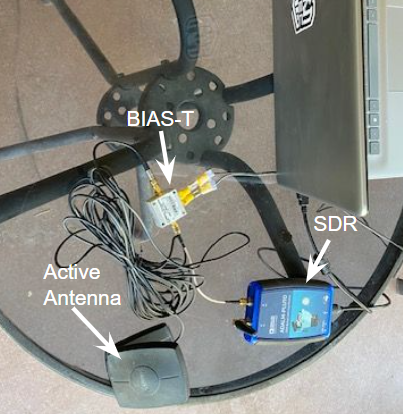
\includegraphics[width=0.5\textwidth]{capture_setup.png}}
	\caption{Hardware Setup for GNU Radio Collection}
	\label{fig::gnu_hardware}
\end{figure}

% We used our Pluto SDR to capture XM radio data using an active antenna in the configuration shown in Figure \ref{fig::active_antenna_setup}.

\subsection{QPSK Demodulation}

After collecting the XM radio signal, we use the flowchart shown in Figure \ref{fig::timing_carrier_sync} to demodulate the received signal. Following the work in the background, we include coarse carrier synchronization, a root raised cosine filter, AGC, symbol synchronization, and fine carrier synchronization. At each stage of processing, we add plots of the constellations and frequency response to visualize the affects of each processing stage. 

\begin{figure}[H]
	\centerline{\fbox{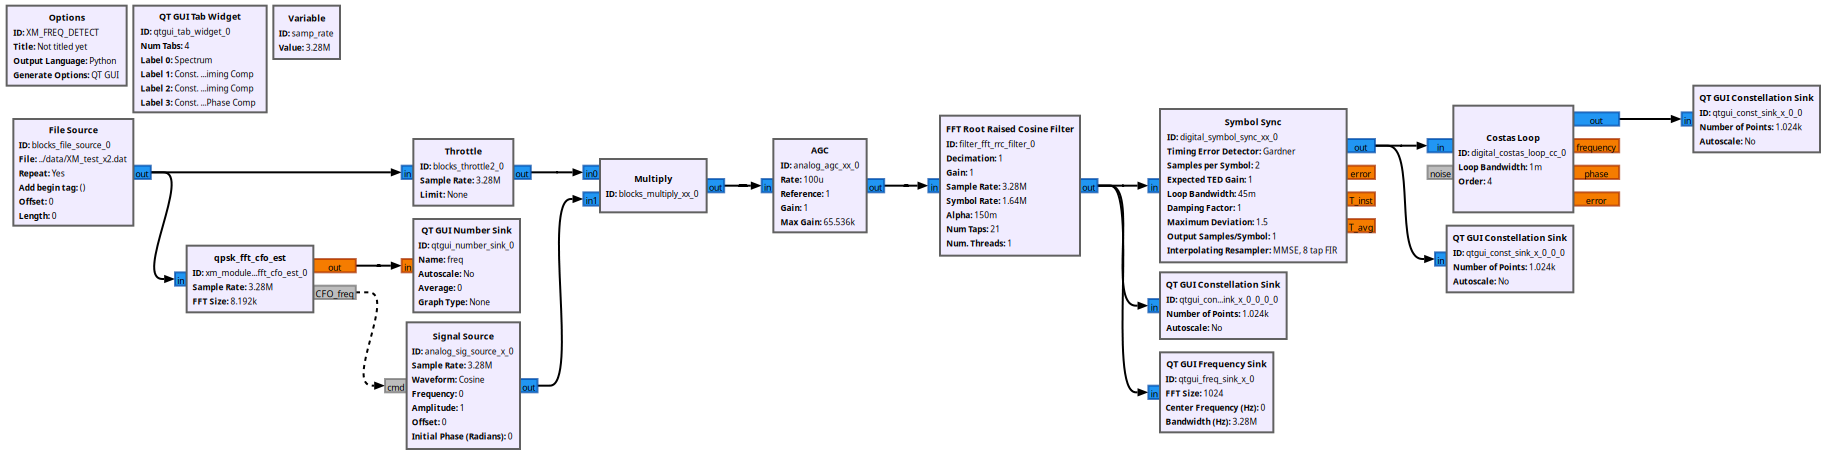
\includegraphics[width=0.9\textwidth]{timing_carrier_sync.png}}}
	\caption{GNU Radio Flowchart for QPSK Demodulation}
	\label{fig::timing_carrier_sync}
\end{figure}

\subsection{Finding the FSP and MFP}

The patents we referenced did not provide the MFP or FSP. As a result, we identified them ourselves using the auto-correlation of our synchronized data. We considered the FSP first because it occurred more frequently in our collected data. To compute the FSP, we selected 32 samples (the FSP duration) and correlated them with a copy of the signal delayed by 3456 samples (the FSP separation). Then, to identify the FSP, we swept our sample selection until the auto correlation was maximized. This approach is illustrated in Figure \ref{fig::finding_fsp}.

\begin{figure}[H]
	\centerline{\fbox{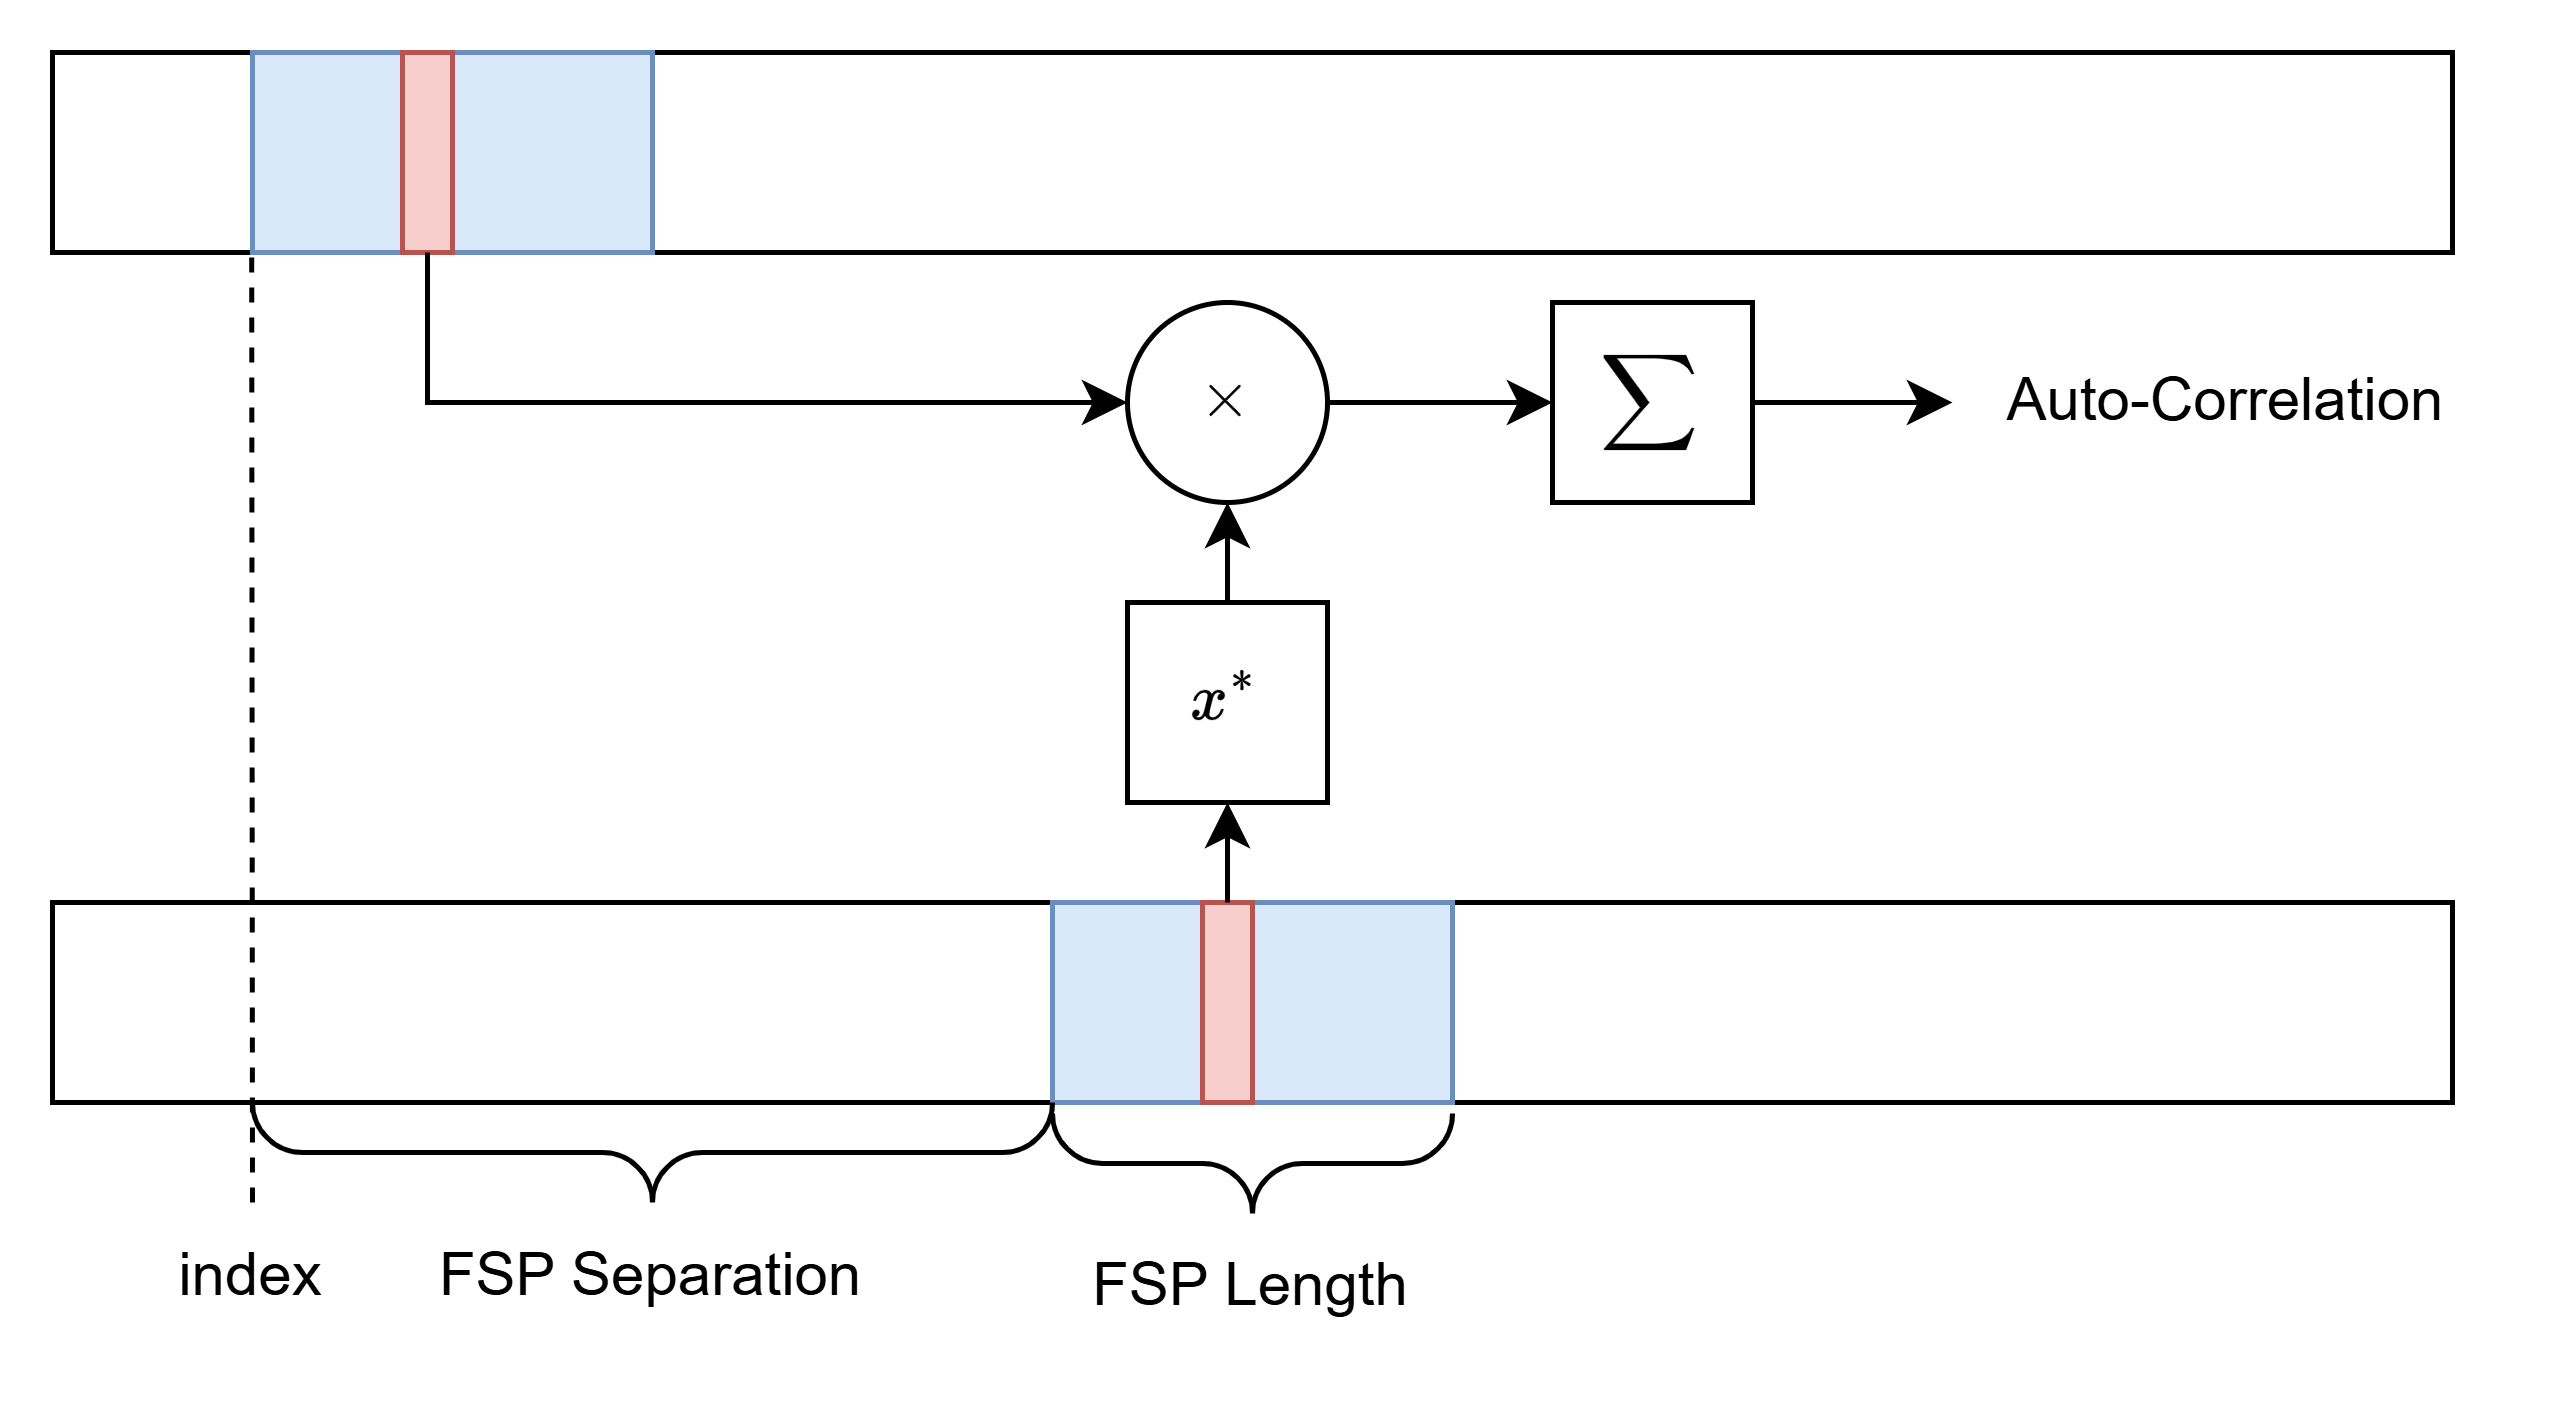
\includegraphics[width=0.5\textwidth]{finding_fsp.png}}}
	\caption{Algorithm for Indentifying FSP}
	\label{fig::finding_fsp}
\end{figure}

We can perform a similar procedure to identify the MFP. However, to reduce the amount of processing, we take advantage of the MFP location illustrated in Figure \ref{fig::tdm_frame_format}. We specifically know that the MFP will always be located right before the FSP. Therefore, we compute the auto-correlation considering these positions only as illustrated in Figure \ref{fig::finding_mfp}.

\begin{figure}[H]
	\centerline{\fbox{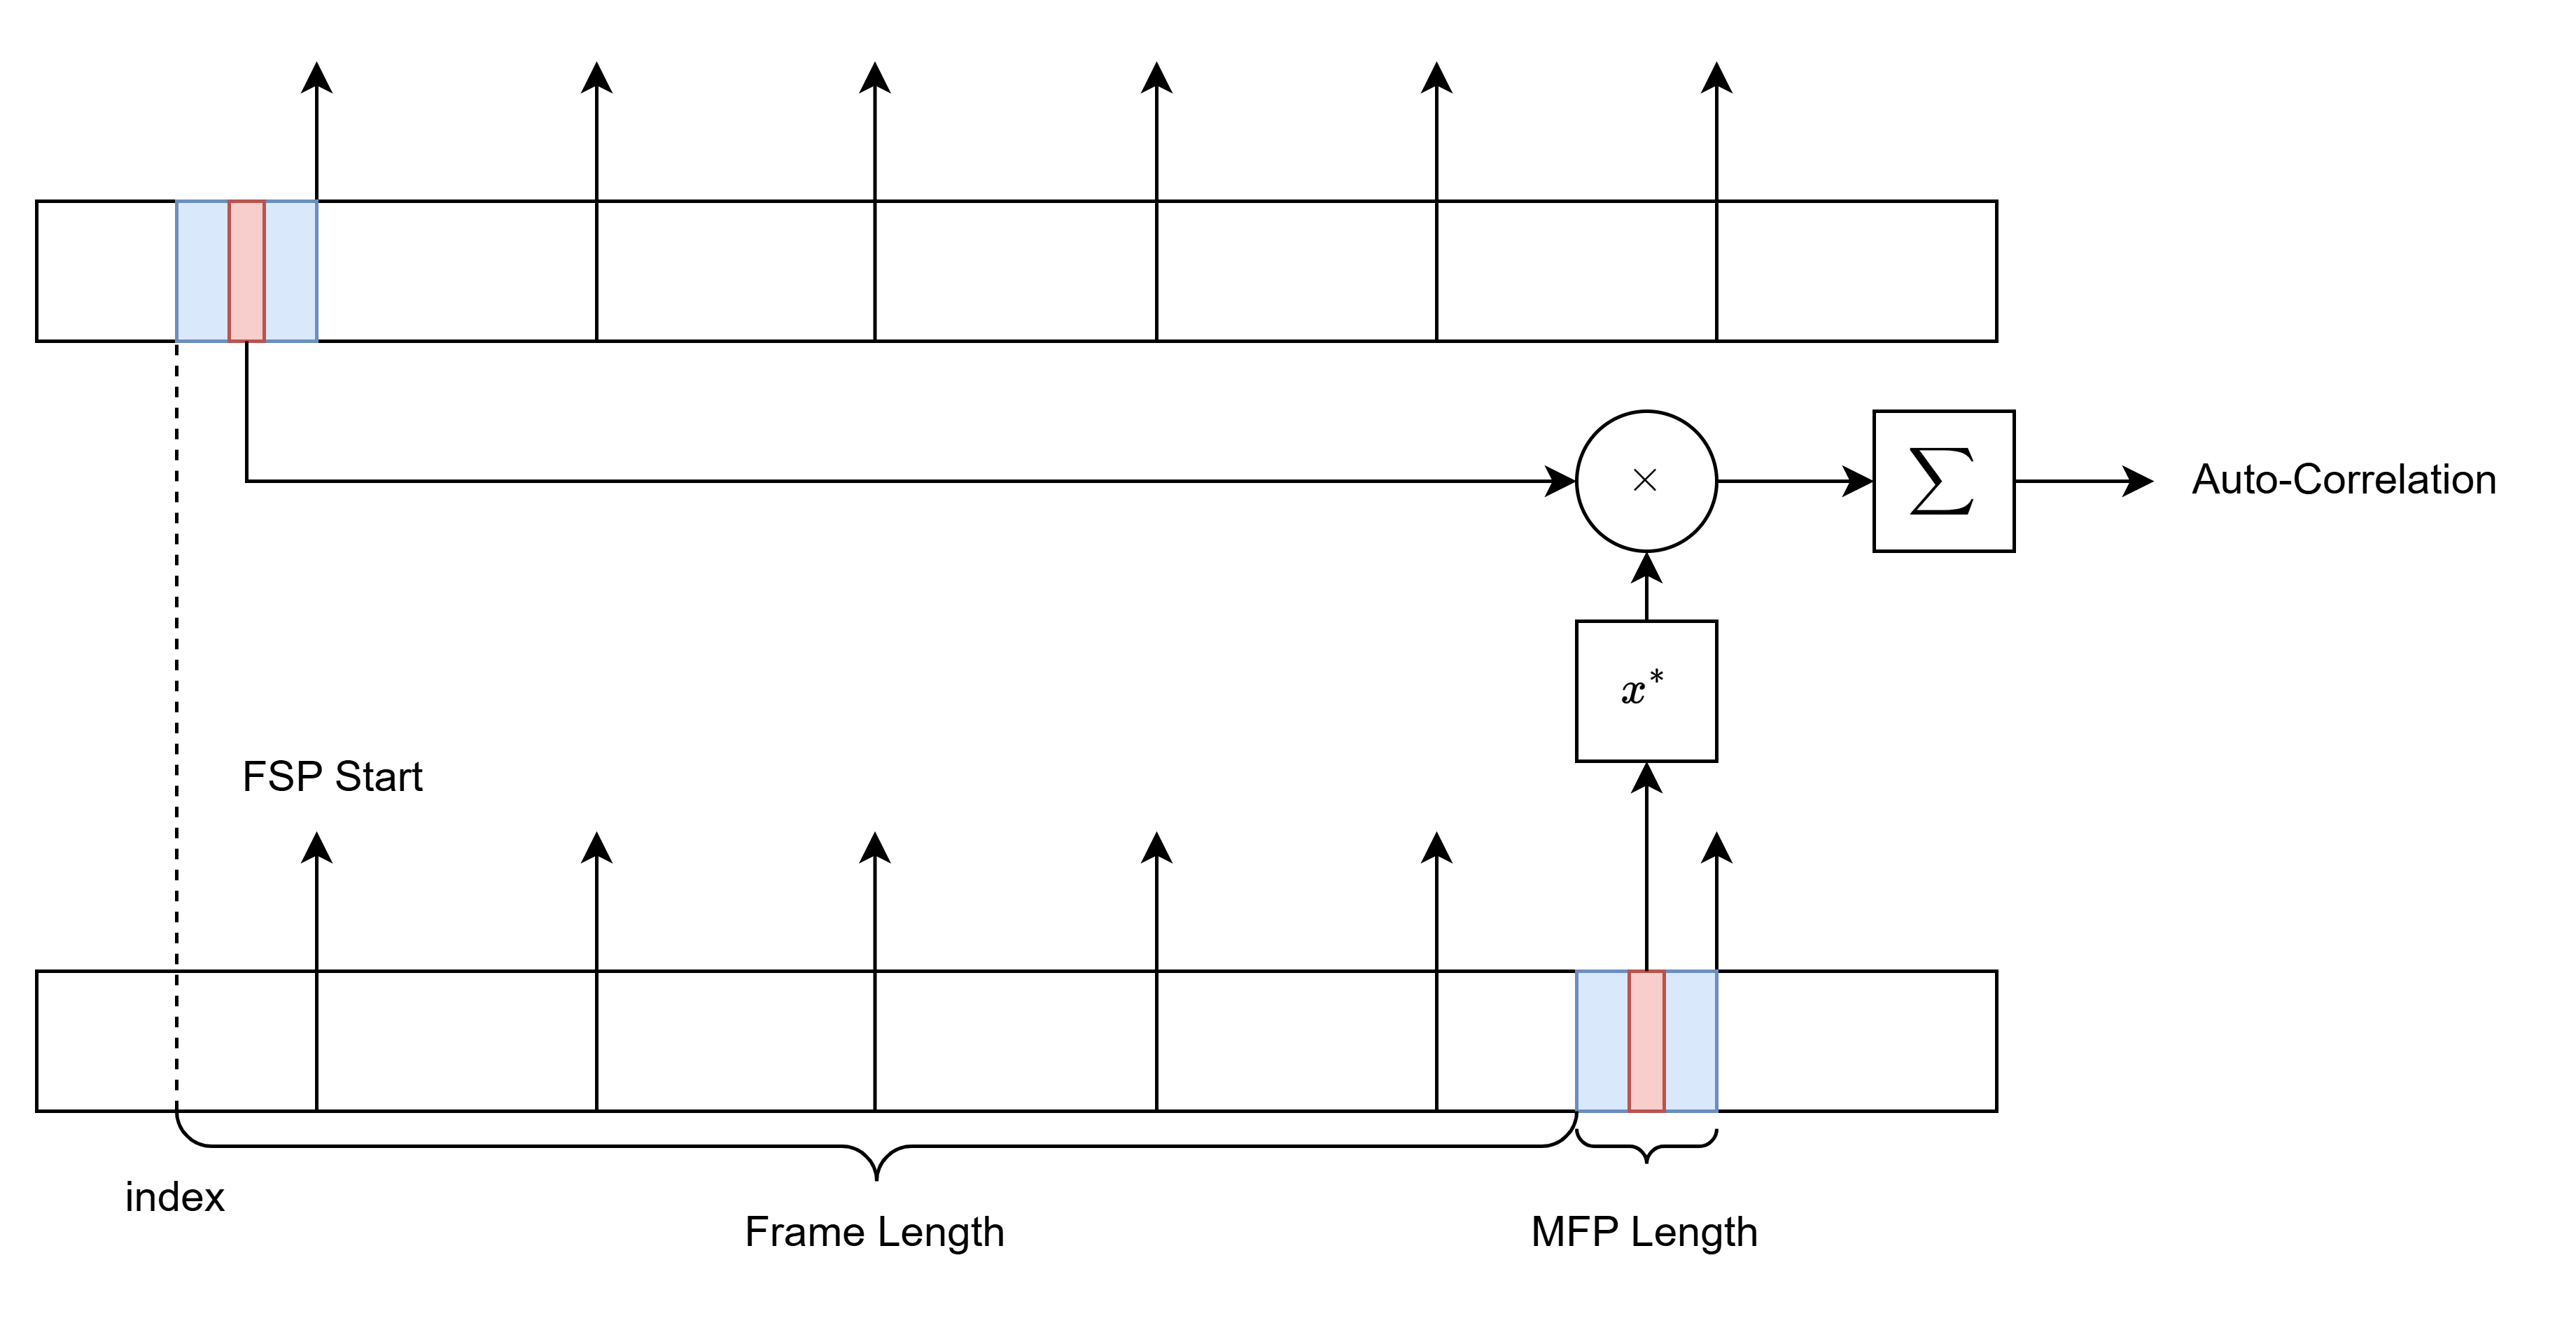
\includegraphics[width=0.5\textwidth]{finding_mfp.png}}}
	\caption{Algorithm for Indentifying MFP}
	\label{fig::finding_mfp}
\end{figure}

\subsection{Convolutional Decoder}

% Once we find the FSP and MFP, we can break our data up into MFP-aligned blocks. We specifically examined the first PRC (5440 bits) of the satellite 2 signal following the description of the time interleaver. The first PRC mentioned at the TSCC (time slot control channel) and should contain a frame counter

After we have the FSP and MFP, we can create MFP aligned blocks of 5440 bits. According to the XM chipset STA400a \cite{alldatasheetcom_2015_sta400a}, there should be a TSCC (time slot control channel) in the first PRC (5440 bits) that contains a frame counter. We specifically consider the first PRC of satellite 2, which we extracted following the description of the time interleaver. Since only one satellite was used, multiple frames were processed through the time interleaver to accumulate enough bits for testing with a Matlab Viterbi decoder.

	% Taking the MFP aligned blocks, the first PRC (5440 bits) of satellite 2 was extracted following the description of the time interleaver.  These are mentioned at the TSCC (time slot control channel) and should contain a frame counter.  This was chosen as the best PRC to use as the channel structure is not expected to change constantly through a shorter time frame.  Because we were examining a single satellite, the time interleaver output to several frames to have enough transmitted bits to test against a Matlab Viterbi decoder.  With a single satellite, one can use either the top portion of the Viterbi decoder or the bottom portion depending on the chosen satellite.  With both satellites, one would chose to run the Viterbi as a rate 1/3 code rate.  With a single satellite one can use a rate 1/2 Viterbi with correct puncturing.  For a single satellite, the effective convolutional encoder rate is 3/4.  I.e. for every 4 received bits, there will be 3 usable information bits.  The decoder needs more than 3 transmission bits in order to determine the state of the trellis.

\subsection{Reed Solomon Decoder}

To familiarize ourselves with the Reed Solomon Decoder, we instantiate a Reed Solomon Decoder in GNU radio and test it with data generated in MATLAB. Our flowchart is shown in Figure \ref{fig::rs_test_grc}. 

\begin{figure}[H]
	\centerline{\fbox{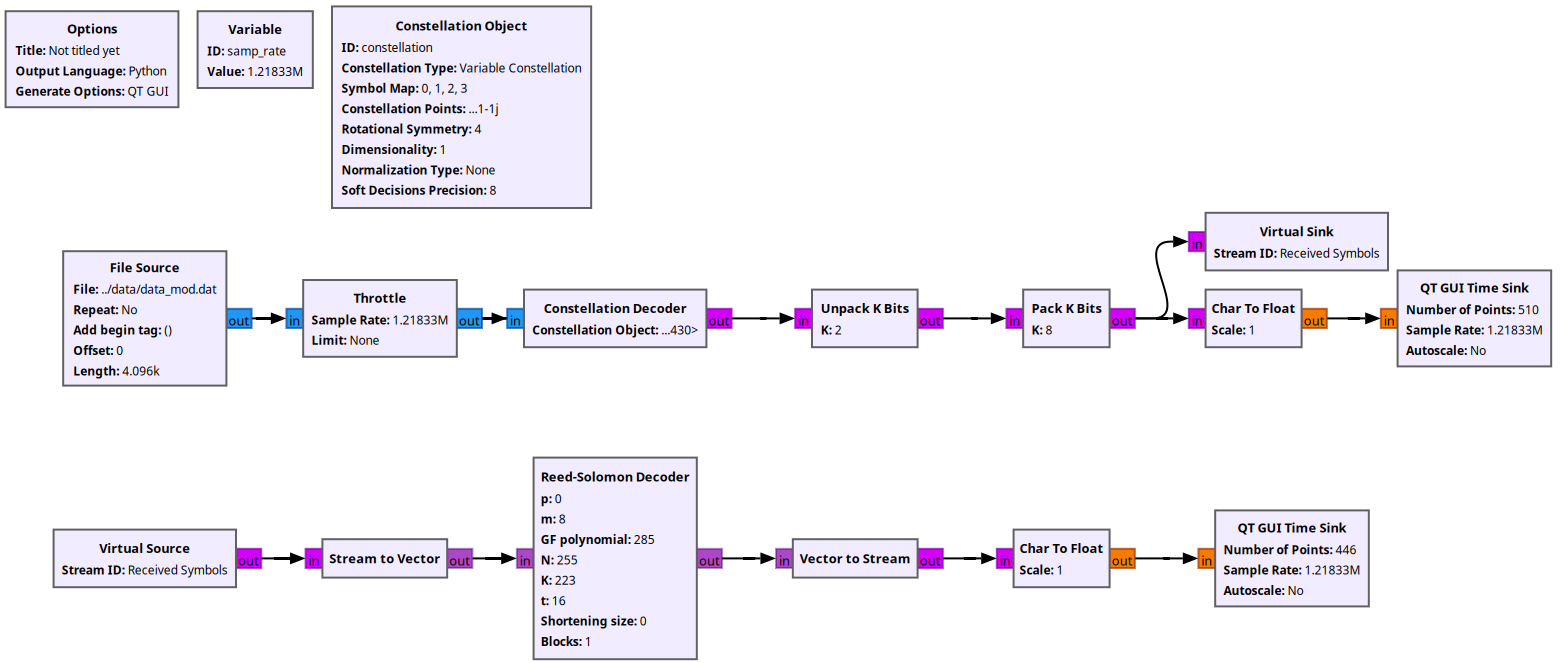
\includegraphics[width=0.8\textwidth]{RS_test_grc.png}}}
	\caption{GRC Flowchart to Test RS Decoder}
	\label{fig::rs_test_grc}
\end{figure}

	Note that for this experiment, we use the DVB-T Reed-Solomon Decoder that is provided by the  Digital Television Library. By default, this decoder uses a (255, 239) RS code (N=255 and K=239) with a shortening size of 51. To make it compatible with the XM radio specification, we let K=223 and set the shortening size to 0. We also set t=16 to correct for the maximum number of errors. Once we have the flowchart working on MATLAB-generated data, we can use it to decode the Viterbi decoder output. To make this transition we simply need to remove the constellation decoder and directly input a stream of bits.

\section{Results}

\subsection{QPSK Demodulation}

In this section, we highlight the results from each of our experiments. We start by analyzing the QPSK demodulator. The spectrum of the received signal before and after applying the root raised cosine (RRC) filter is shown in Figure \ref{fig::root_raised_cosine_spectrum}.

\begin{figure}[H]
	\centerline{\fbox{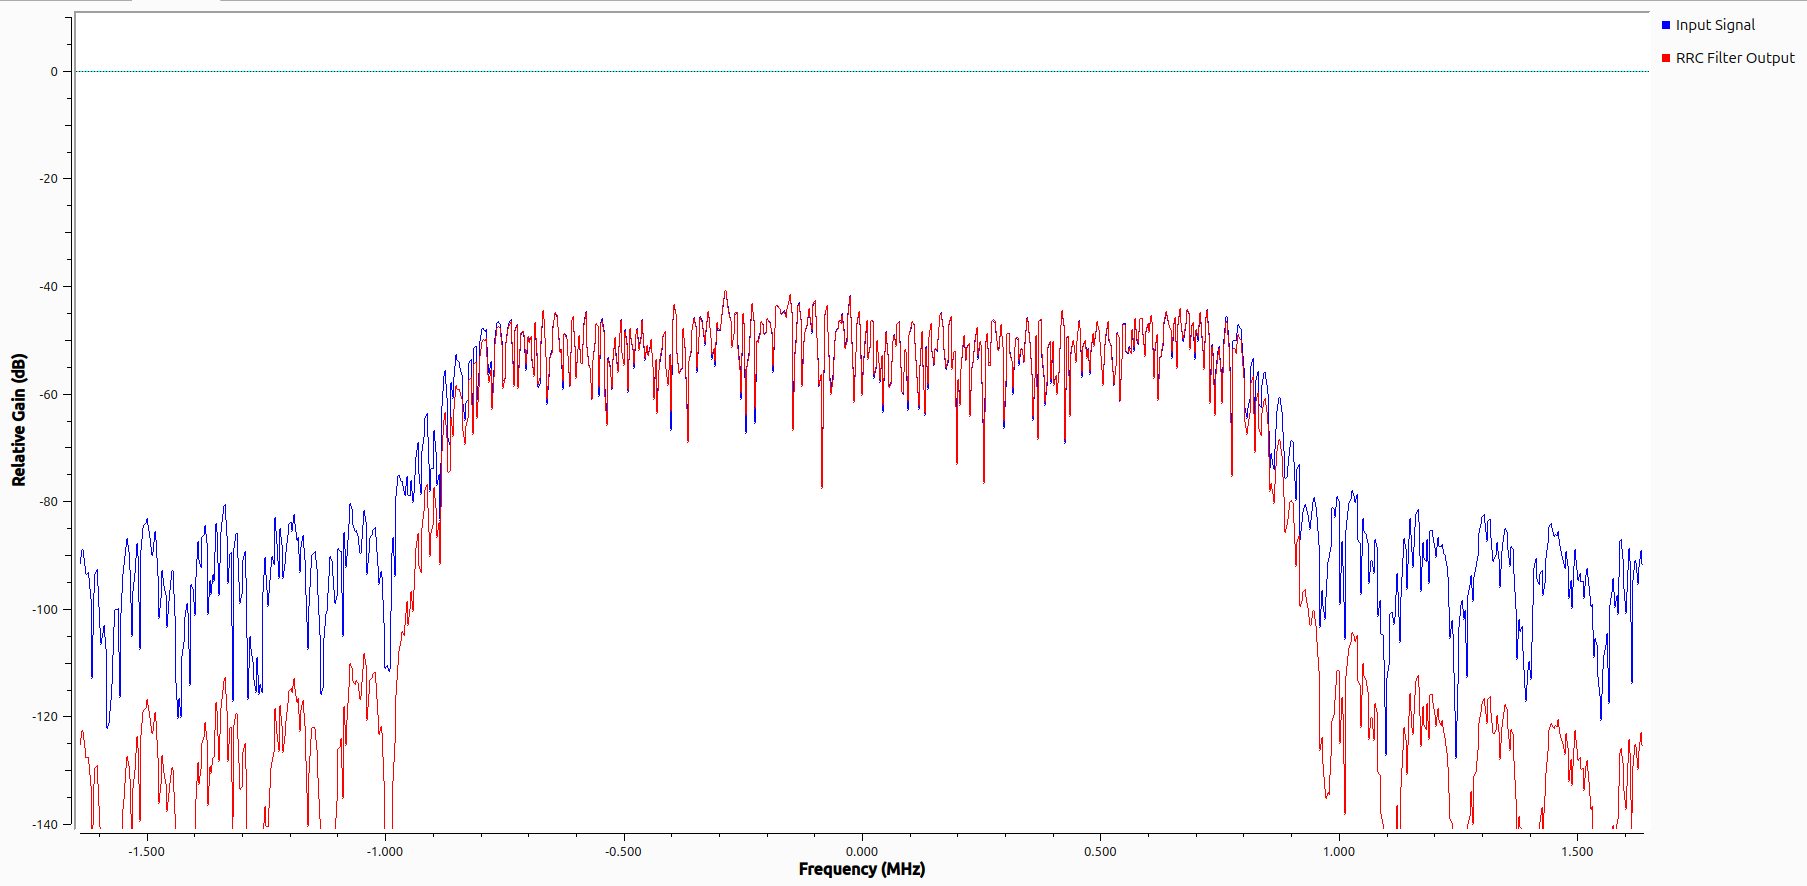
\includegraphics[width=0.5\textwidth]{root_raised_cosine_spectrum.png}}}
	\caption{Spectrum Before and After Apply Root-Raised Cosine Filter}
	\label{fig::root_raised_cosine_spectrum}
\end{figure}

\noindent As previously discussed, the RRC filter is a type II Nyquist filter, so it should result in zero ISI when the signal is sampled at the midpoint of the symbol transitions. In practice, we cannot enforce this timing, and we get the constellation shown in Figure \ref{fig::constellation_no_timing_comp}.

\begin{figure}[H]
	\centerline{\fbox{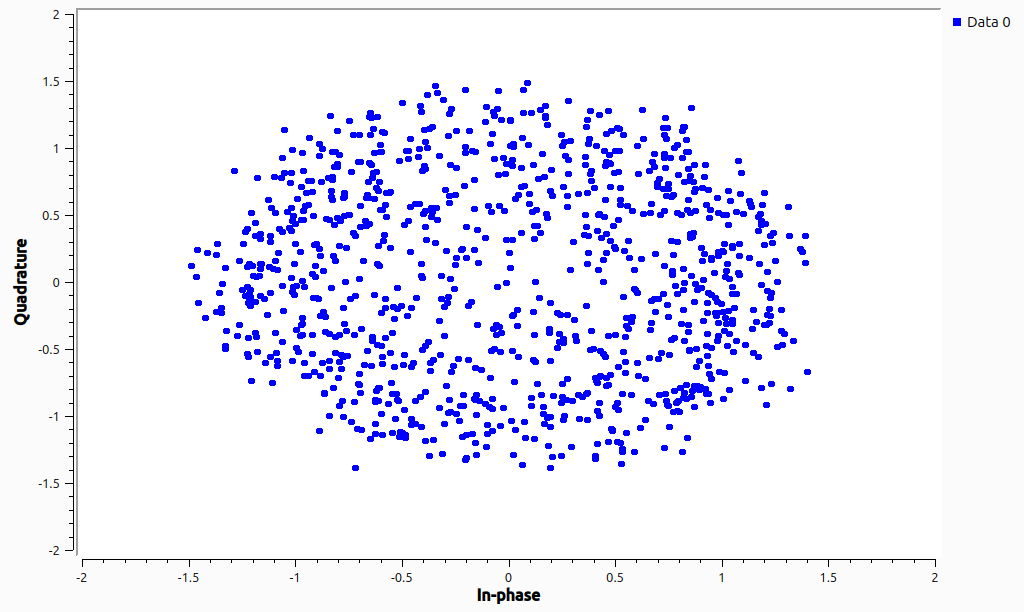
\includegraphics[width=0.5\textwidth]{constellation_no_timing_comp.png}}}
	\caption{Received Constellation Before Timing Synchronization}
	\label{fig::constellation_no_timing_comp}
\end{figure}

\noindent We perform timing compensation to correct for the imperfect sampling. To do this we leverage GNU radio's symbol sync block, which contains an interpolator, timing error detector, loop filter, and controller. For our work, we specifically configure the block to use a Gardner Timing Error detector because it is robust to frequency errors. Our constellation after timing compensation is shown in Figure \ref{fig::constellation_after_timing_comp}.

\begin{figure}[H]
	\centerline{\fbox{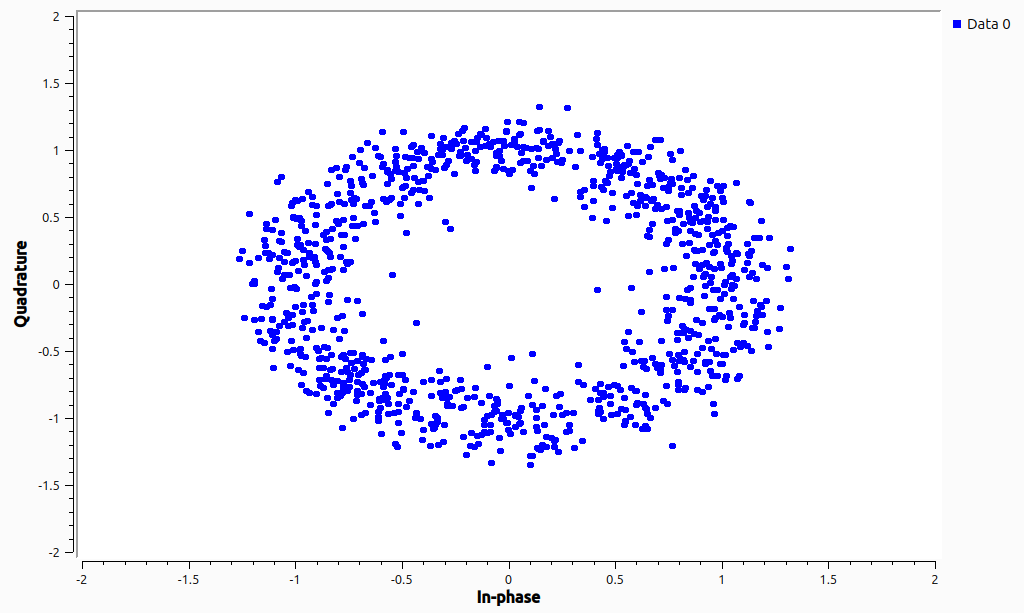
\includegraphics[width=0.5\textwidth]{constellation_after_timing_comp.png}}}
	\caption{Received Constellation After Timing Synchronization}
	\label{fig::constellation_after_timing_comp}
\end{figure}

After timing compensation, we see that the amplitude of the constellation has stabilized. However, the resulting constellation is a ring. This occurs because of phase and frequency errors. The phase error leads to a static tilt of the constellation, and the frequency offset causes our constellation to rotate. To correctly demodulate the signal, we must also remove the frequency offset in the signal. We do this in 2 stages: coarse frequency compensation and fine frequency compensation. We implement coarse frequency compensation in a custom GNU radio python block, which implements the algorithm given in Equation \ref{eq::cfo_estimate}. The FFT output and the corresponding coarse frequency offset (CFO) are shown in Figure \ref{fig::cfo_frequency_estimate}. Examining the Figure, we observe a frequency error of roughly 15 kHz.

\begin{figure}[H]
	\centerline{\fbox{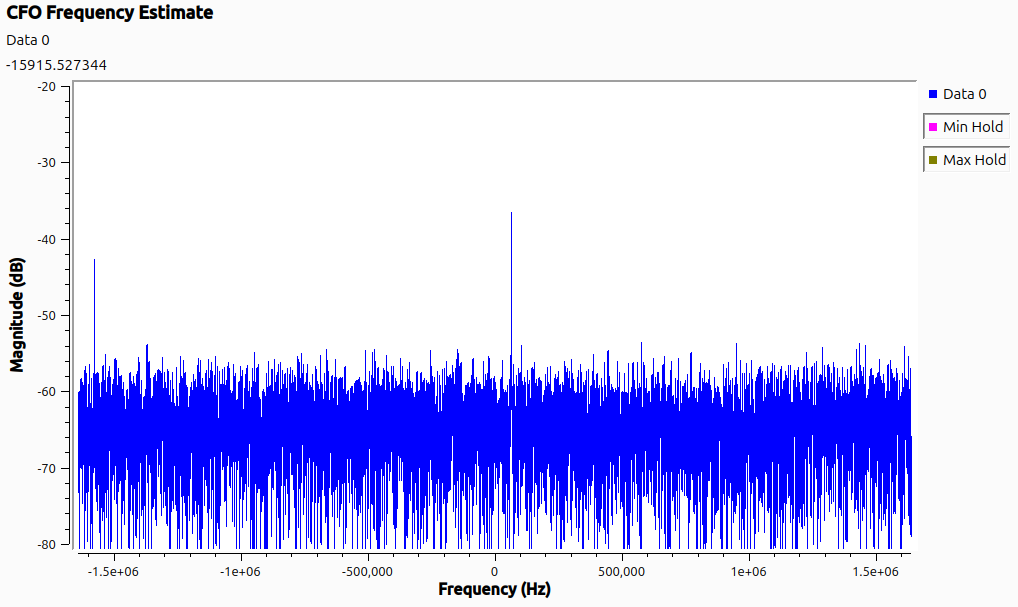
\includegraphics[width=0.5\textwidth]{cfo_frequency_estimate.png}}}
	\caption{Coarse Frequency FFT Output}
	\label{fig::cfo_frequency_estimate}
\end{figure}

The coarse frequency compensation is limited by the FFT size and the rate at which the frequency drifts. We add an additional fine frequency compensation block to resolve the rest of the error. We use the GNU radio Costas Loop block for this analysis. The GNU radio Costas Loop block implements a algorithm similar to the fine carrier compensation block. It includes a phase error detector, a loop filter, a direct digital synthesizer and a phase rotator. The constellation after fine frequency compensation is shown in Figure \ref{fig::constellation_after_fine_carrier_comp}.

\begin{figure}[H]
	\centerline{\fbox{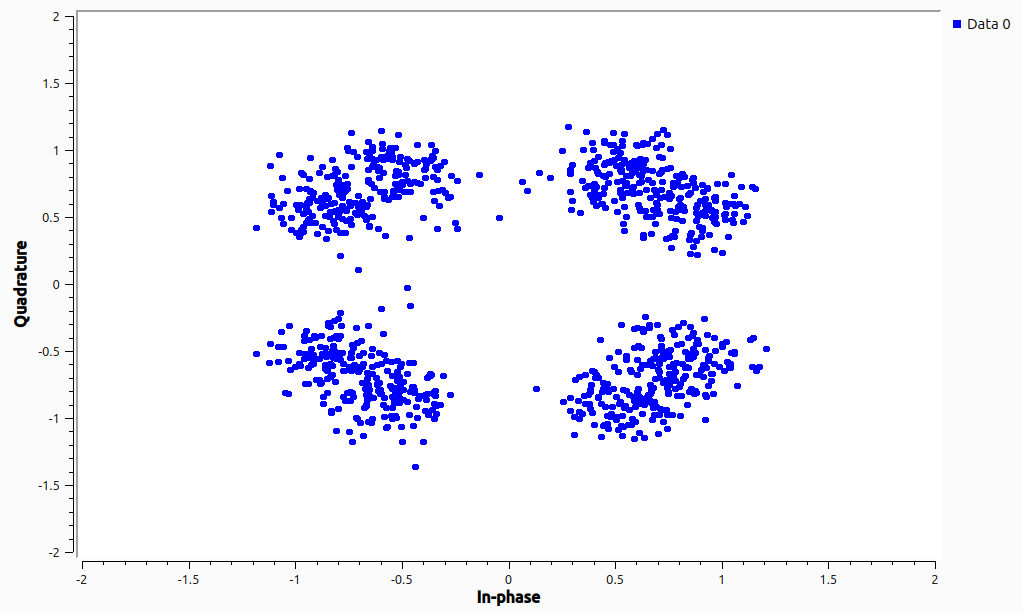
\includegraphics[width=0.5\textwidth]{constellation_after_fine_carrier_comp.png}}}
	\caption{Received Constellation After Fine Carrier Synchronization}
	\label{fig::constellation_after_fine_carrier_comp}
\end{figure}

\noindent After carrier synchronization, the constellation cleans up and we see the QPSK symbols with a PSK hierarchical modulation of $\pm15^{\circ}$. For the purposes of this report, we ignore the hierarchical modulation and consider only the QPSK symbols. In this configuration, we can treat the hierarchical modulation as "additional phase noise".

% The XM radio signal is transmitted through a square-root raised cosine filter, which limit the signal bandwidth [ADD A CITATION HERE]. Because of this, the receiver needs a matching square root raised cosine filter. The root-raised cosine filter is a type II Nyquist filter, which results in zero intersymbol interference when the received signal is sampled at the midpoint of each symbol period. When the PlutoSDR samples the received signal, this condition is not strictly enforced. This results in significant spreading in our constellation as illustrated in Figure \ref{fig::constellation_no_timing_comp}.

%\begin{figure}[H]
%	\centerline{\fbox{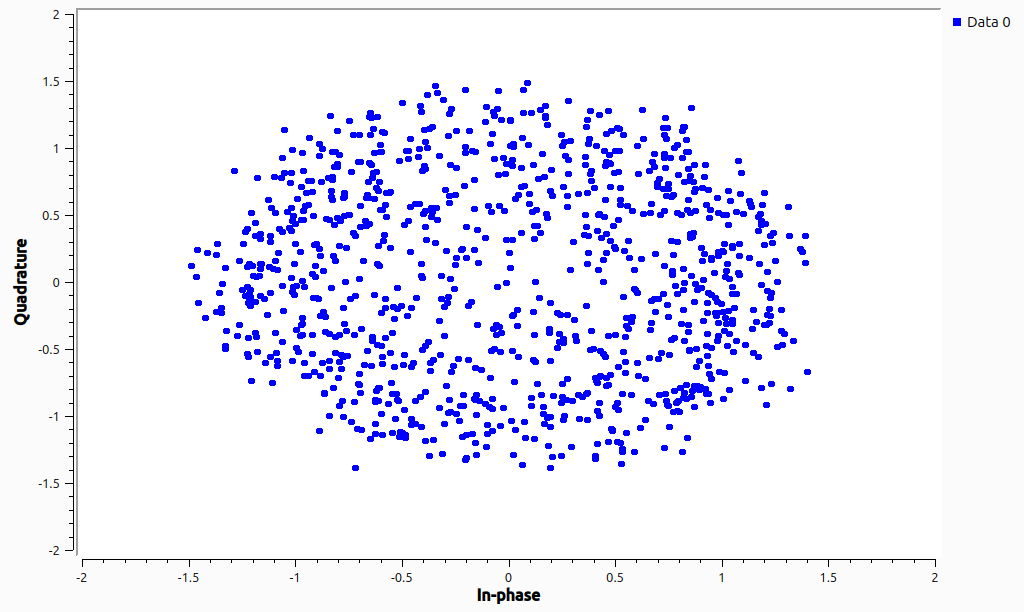
\includegraphics[width=0.5\textwidth]{constellation_no_timing_comp.png}}}
%	\caption{Received Constellation Before Timing Synchronization}
%	\label{fig::constellation_no_timing_comp}
%\end{figure}

%We can correct for this timing offset using a timing synchronization block. For this purpose, we use a GNU radio symbol sync block. This symbol sync block can be subdivided into 4 blocks: interpolator, timing error detector, loop filter, and controller. The interpolator applies a fractional delay. The timing error detector measures the timing offset. The loop filter stabilizes the process. And the controller manages the interpolation process. For our work, we specifically choose a Gardner Timing Error detector because it is robust to frequency errors. Our constellation after timing compensation is shown in Figure \ref{fig::constellation_after_timing_comp}.

%\begin{figure}[H]
%	\centerline{\fbox{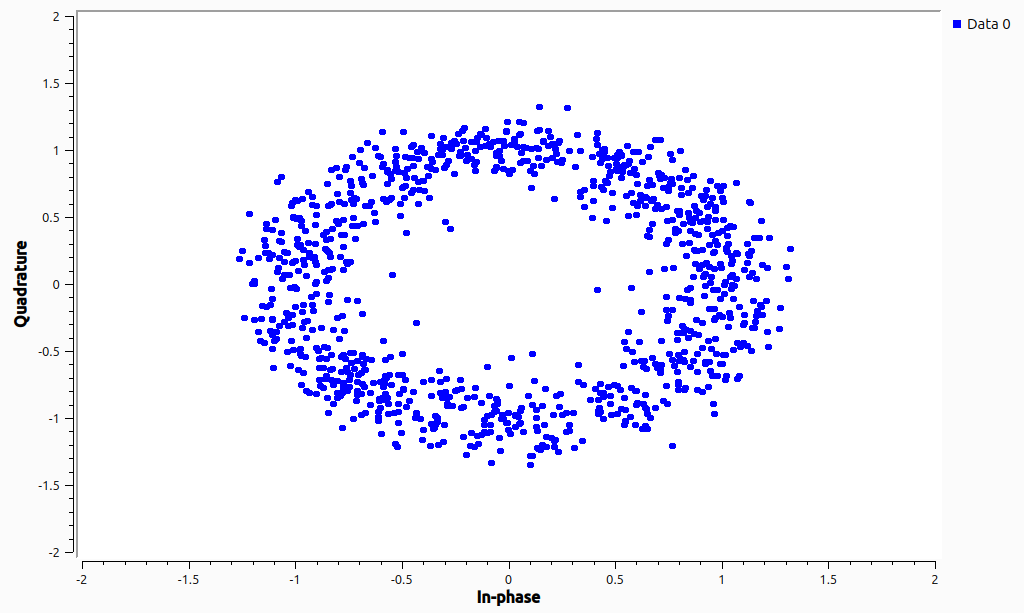
\includegraphics[width=0.5\textwidth]{constellation_after_timing_comp.png}}}
%	\caption{Received Constellation After Timing Synchronization}
%	\label{fig::constellation_after_timing_comp}
%\end{figure}

%After timing compensation, we see that the amplitude of the constellation has stabilized. However, the resulting constellation is a ring. This occurs because after phase and frequency errors. The phase error leads to a static tilt of the constellation and the frequency offset causes our constellation to rotate. To correctly demodulate the signal, we must also remove the frequency offset in the signal. We do this in 2 stages: coarse frequency compensation and fine frequency compensation. We implement the coarse frequency compensation algorithm using a custom GNU radio python block. This block raises our received data to the fourth power to remove the QPSK modulation. Then, it takes an FFT of the resulting signal. The peak index of the FFT provides us with an estimate of the coarse frequency error. When solving for the error we also must divide the frequency error by 4 to account for raising the received data to the 4th power prior to the FFT. The FFT output and the corresponding frequency error for one frame of data is shown in Figure \ref{fig::cfo_frequency_estimate}. Examining the Figure, we observe a frequency error of roughly 15 kHz [CHECK SIGN].

%\begin{figure}[H]
%	\centerline{\fbox{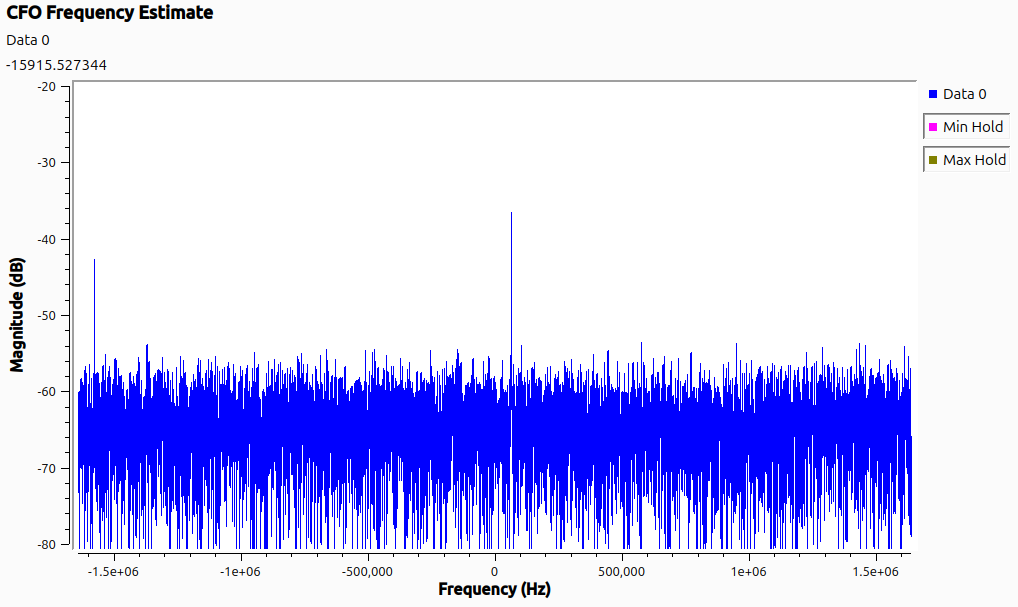
\includegraphics[width=0.5\textwidth]{cfo_frequency_estimate.png}}}
%	\caption{Coarse Frequency FFT Output}
%	\label{fig::cfo_frequency_estimate}
%\end{figure}

% The coarse frequency compensation is limited by the FFT size and the rate at which the frequency drifts. We add an additional fine frequency compensation block to resolve the rest of the error. We use the GNU radio Costas Loop block for this analysis. The GNU radio Costas Loop closely resembles the timing synchronization block. It includes a phase error detector, a loop filter, a direct digital synthesizer and a phase rotator. The phase rotator adjusts the phase of the received signal by multiplying it with a phasor. The phase error detector then detects the phase error, which is fed into a loop filter for stabilization. Finally the Direct Digital Synthesizer creates a coherent phasor which removes residual phase and frequency offsets. The constellation after fine frequency compensation is shown in Figure \ref{fig::constellation_after_fine_carrier_comp}.

%\begin{figure}[H]
%	\centerline{\fbox{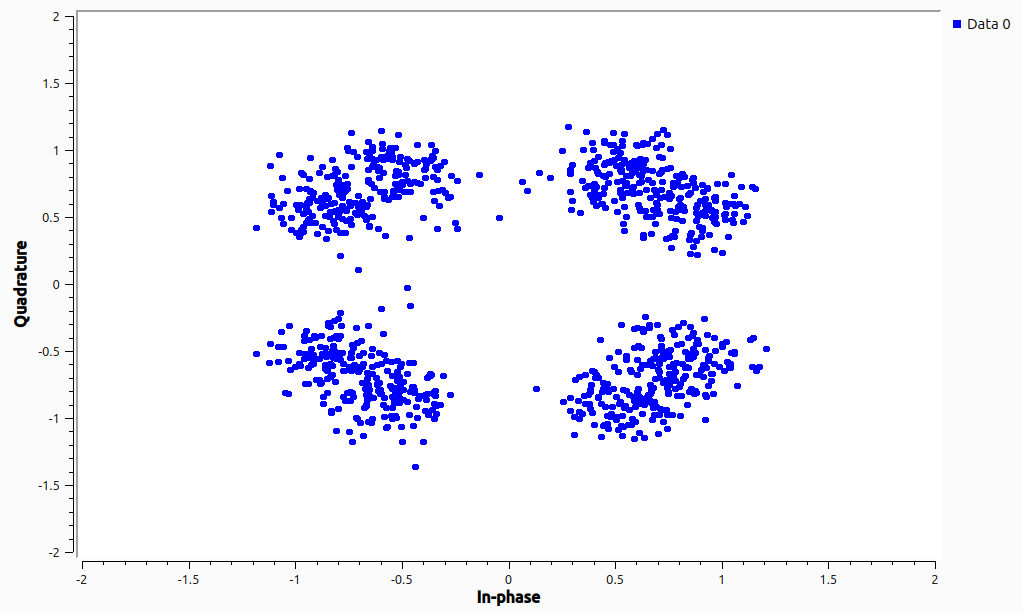
\includegraphics[width=0.5\textwidth]{constellation_after_fine_carrier_comp.png}}}
%	\caption{Received Constellation After Fine Carrier Synchronization}
%	\label{fig::constellation_after_fine_carrier_comp}
%\end{figure}

\subsection{Finding the FSP and MFP}

In this section, we compute the FSP and MFP using the algorithms illustrated in Figures \ref{fig::finding_fsp} and \ref{fig::finding_mfp} respectively. In Figure \ref{fig::fsp_correlation}, we show the peak FSP auto-correlation.

\begin{figure}[H]
	\centerline{\fbox{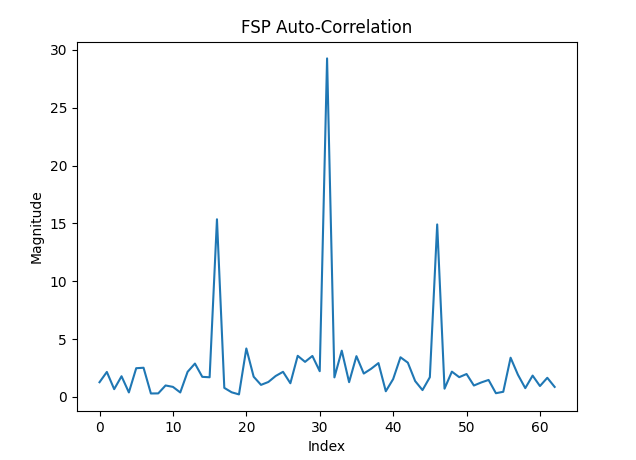
\includegraphics[width=0.5\textwidth]{fsp_correlation.png}}}
	\caption{Auto-Correlation of Optimum FSP Selection}
	\label{fig::fsp_correlation}
\end{figure}

\noindent We can use the peak location of the auto-correlation output to determine the location of the FSP in our data. In Figure \ref{fig::fsp_constellation}, We show the constellation for our FSP samples against the contellation points for the rest of the symbols in the payload.

\begin{figure}[H]
	\centerline{\fbox{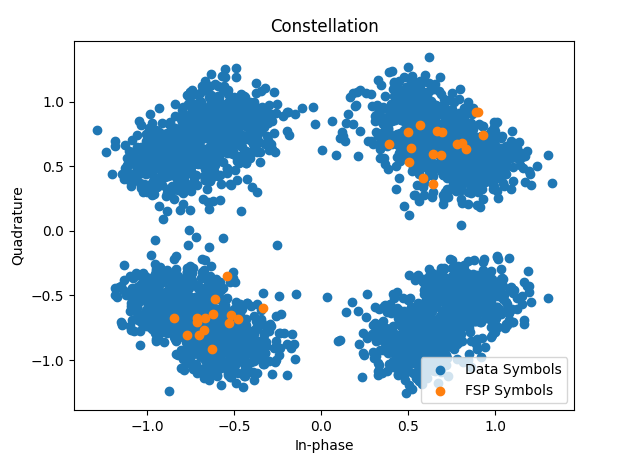
\includegraphics[width=0.5\textwidth]{fsp_constellation.png}}}
	\caption{Constellation of FSP Symbols vs Data Symbols}
	\label{fig::fsp_constellation}
\end{figure}

\noindent Examining the constellation, we see that the FSP is using BPSK modulation with a phase rotation of $45^{\circ}$. If we demodulate each of our points, we can create a noise-free estimate of our FSP. Note that the resulting FSP is ambiguous by $90n^{\circ}$, where $n \in \mathcal{Z}$. This is not important for detecting the start of frames, but is important for applications such as EQ.

We can apply a similar algorithm to find the MFP. However, we now only consider the possible MFP positions (right before the FSP). Doing so, significantly reduces the computation time. The peak MFP auto-correlation is shown in Figure \ref{fig::mfp_correlation}.

\begin{figure}[H]
	\centerline{\fbox{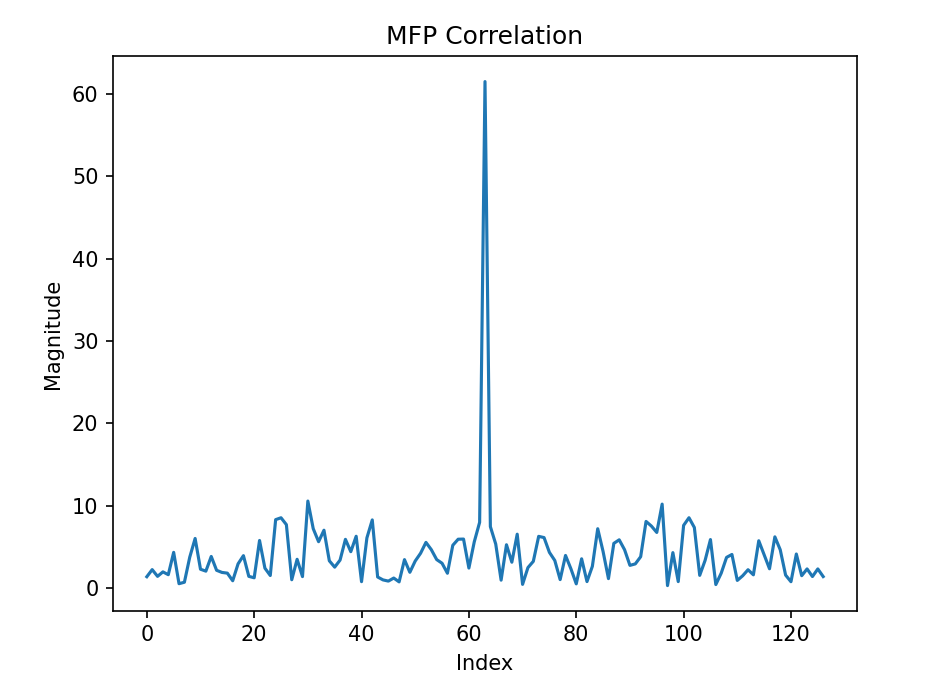
\includegraphics[width=0.5\textwidth]{mfp_correlation.png}}}
	\caption{Auto-Correlation of Optimum MFP Selection}
	\label{fig::mfp_correlation}
\end{figure}

\noindent As we did for the FSP, we can use the peak location of the auto-correlation output to determine the location of the MFP. In Figure \ref{fig::mfp_constellation}, we extract the constellation for our MFP and plot it alongside the constellation for the rest of the preamble.

\begin{figure}[H]
	\centerline{\fbox{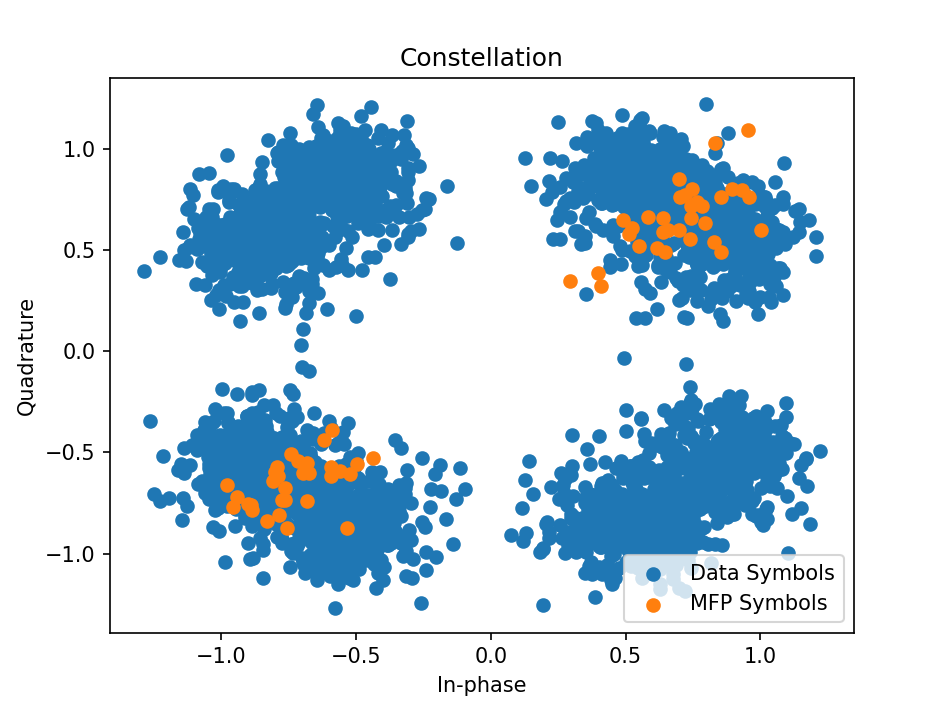
\includegraphics[width=0.5\textwidth]{mfp_constellation.png}}}
	\caption{Constellation of MFP Symbols vs Data Symbols}
	\label{fig::mfp_constellation}
\end{figure}

\noindent Similar to the FSP, we see that the MFP is using BPSK modulation with a phase rotation of $45^{\circ}$. If we demodulate each of our points, we can create a noise-free estimate of our MFP. Note that the resulting MFP is also ambiguous by $90n^{\circ}$, where $n \in \mathcal{Z}$. This is not important for detecting the start of frames, but is important for applications such as EQ.

We can also update our flowchart to cross-correlate our received data with the FSP and MFP. By thresholding the peaks of the correlation, we can output only the aligned data bits, which will be fed into the FEC algorithms. In our initial approach this was done with standalone python scripts. However, this is an incremental step in creating a GNU Radio flowchart for the entire system. The updated flowchart is shown in Figure \ref{fig::frame_align}.

\begin{figure}[H]
	\centerline{\fbox{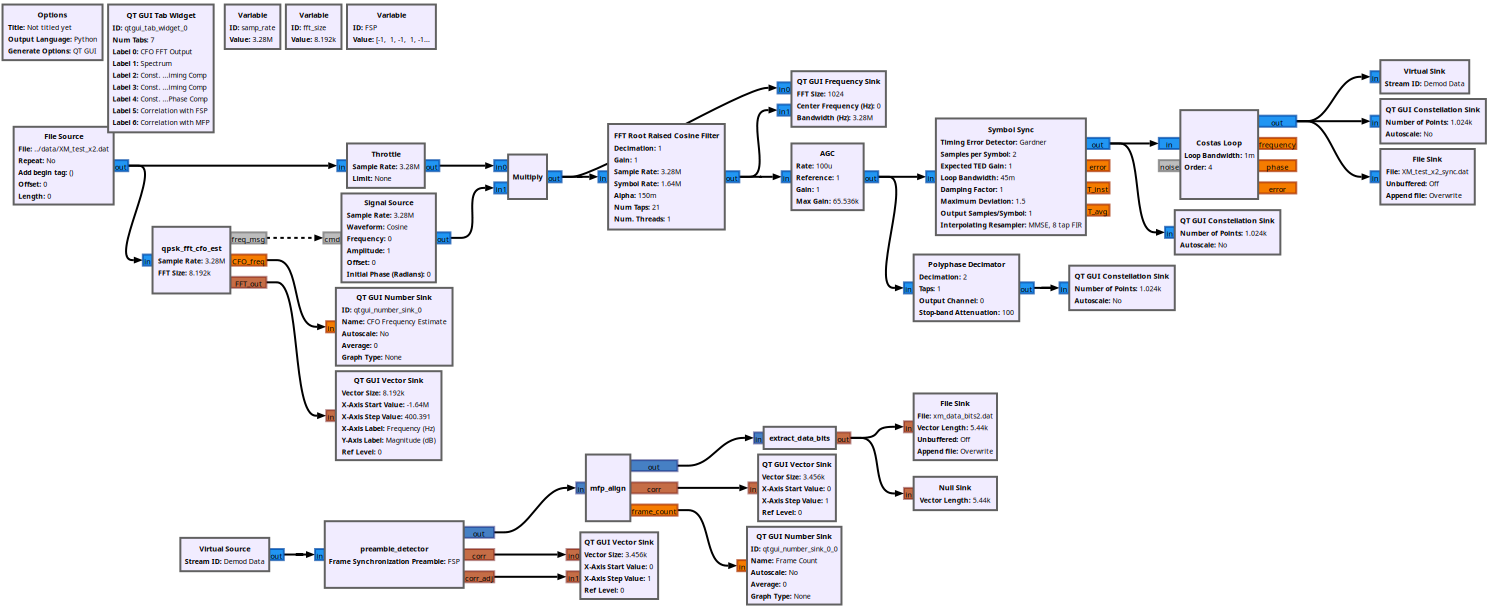
\includegraphics[width=0.9\textwidth]{frame_align.png}}}
	\caption{Updated GNU Flowchart that Outputs Only the Aligned Data Bits}
	\label{fig::frame_align}
\end{figure}

The first new block in our flowchart correlates the input data with the FSP and aligns the data such that the FSP shows up at the start of the frame. The second block correlates the signal with the MFP and outputs the data only when the first MFP immediately proceeds the frame. In Figure \ref{fig::fsp_correlation_gnu_radio}, we have attached the cross-correlation results with the FSP. We also show the FSP position after frame alignment. Note that the correlation peak after alignment occurs at sample 31 instead of sample 0 because we are using the \texttt{filter} command for correlation.

\begin{figure}[H]
	\centerline{\fbox{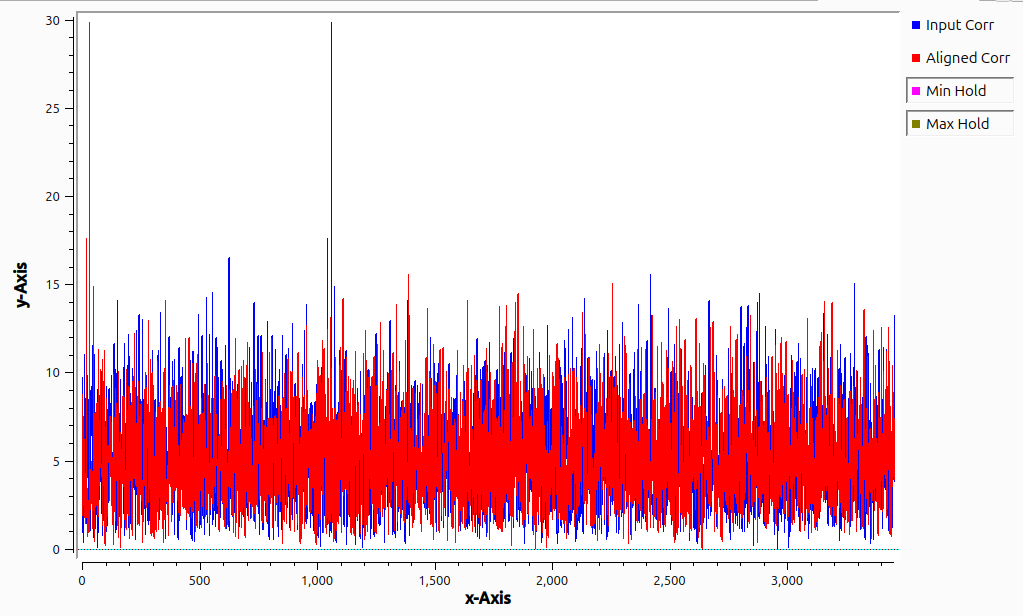
\includegraphics[width=0.5\textwidth]{fsp_correlation_gnu_radio.png}}}
	\caption{Correlation of Input Data with FSP Before and After Frame Alignment}
	\label{fig::fsp_correlation_gnu_radio}
\end{figure}

We have also included correlation results with the MFP, which are attached in Figure \ref{fig::fsp_correlation_gnu_radio}. Note that the correlation peak occurs on the last sample because the MFP is placed at the end of each frame and because we are using the \texttt{filter} command instead of the \texttt{xcorr} command.

\begin{figure}[H]
	\centerline{\fbox{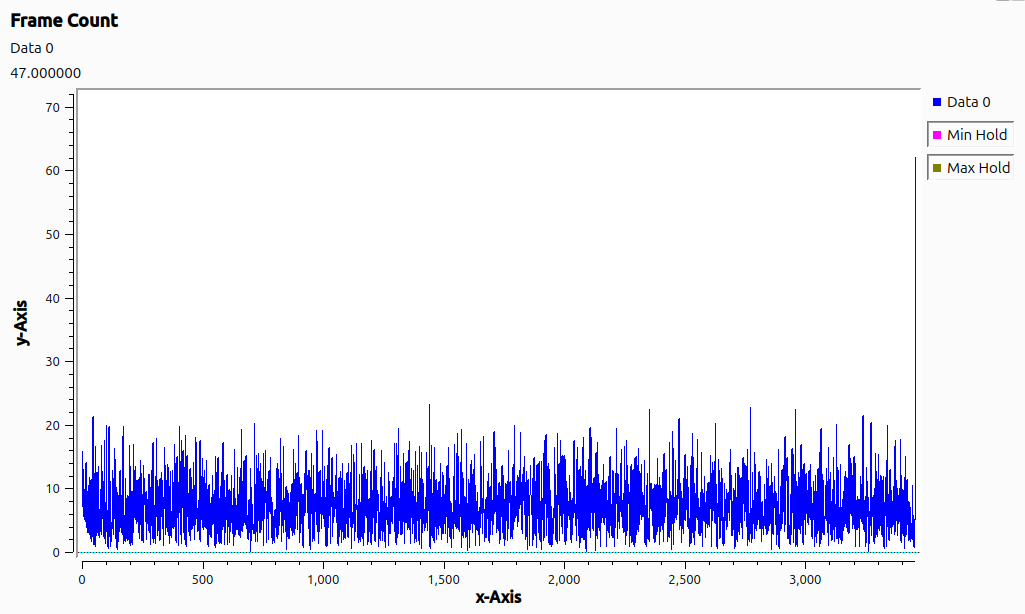
\includegraphics[width=0.5\textwidth]{mfp_correlation_gnu_radio.png}}}
	\caption{Correlation of Aligned Data with MFP}
	\label{fig::mfp_correlation_gnu_radio}
\end{figure}

% \noindent Examining the figure, we see that the MFP XM radio divides its transmitted data into frames. These frames are marked by two different preambles: the MFP (master frame preamble) and the FSP (fast synchronization preamble). The FSP marks the start of the data portion and corrects for ambiguities, while the MFP is used to align the signal from each satellite \cite{a2008_us8260192b2}. Both preambles and their relative timing are illustrated in Figure \ref{fig::tdm_frame_format}.

%\begin{figure}[H]
%	\centerline{\fbox{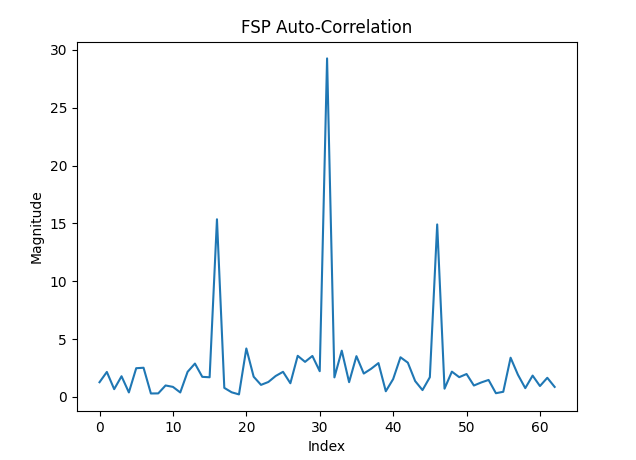
\includegraphics[width=0.5\textwidth]{fsp_correlation.png}}}
%	\caption{Auto-Correlation of Optimum FSP Selection}
%	\label{fig::fsp_correlation}
%\end{figure}

%We can also examine some of the properties of the FSP by looking at its constellation. In Figure \ref{fig::fsp_constellation}, we show the constellation of the FSP symbols and data symbols.

%\begin{figure}[H]
%	\centerline{\fbox{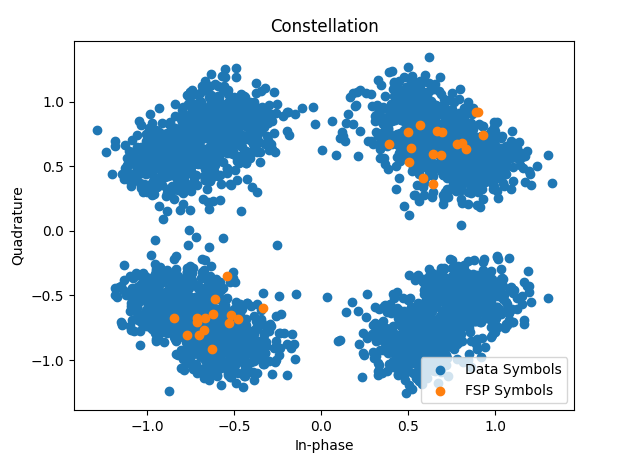
\includegraphics[width=0.5\textwidth]{fsp_constellation.png}}}
%	\caption{Constellation of FSP Symbols vs Data Symbols}
%	\label{fig::fsp_constellation}
%\end{figure}

%Examining the figure, we see that the FSP uses bi-phase modulation (phase-shifted BPSK) instead of QPSK modulation like the proceeding signals. To improve our correlation performance going forward, we demodulate each of the FSP constellation points. Note that our results are ambiguous by $180^{\circ}$, so we assume a leading 1 in the FSPs. Errors reported by the Reed Solomon decoder (when implemented) can be used to resolve this ambiguity. If we receive high error counts, we know to rotate the phase of our FSP by $180^{\circ}$.

% The base case auto-correlation provides the location of the MFP. For our data, the best case auto-correlation is shown in Figure \ref{fig::mfp_correlation} and the resulting constellation is shown in Figure \ref{fig::mfp_constellation}.

%\begin{figure}[H]
%	\centerline{\fbox{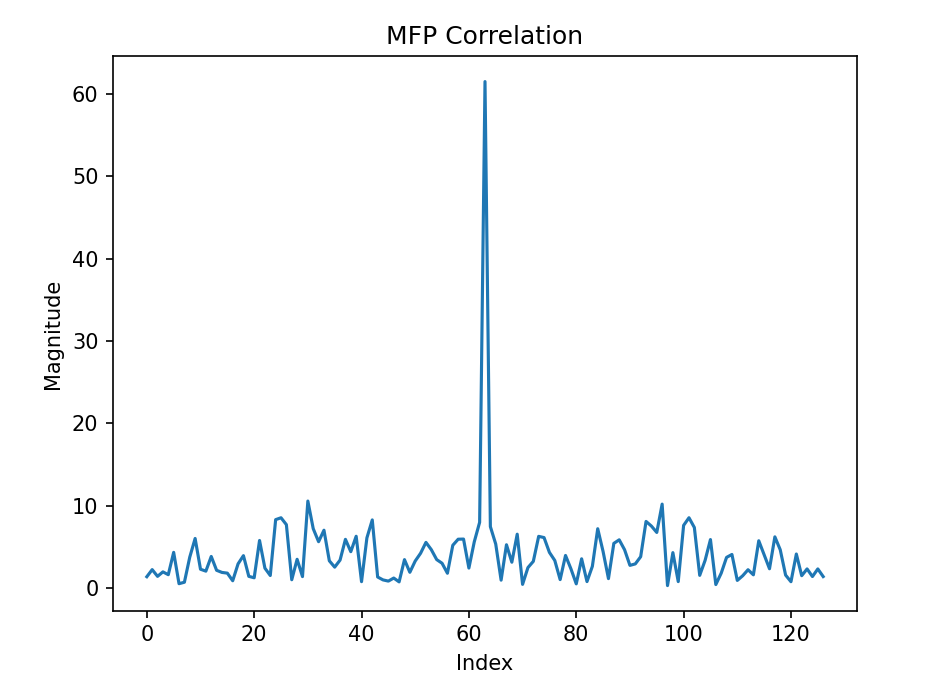
\includegraphics[width=0.5\textwidth]{mfp_correlation.png}}}
%	\caption{Auto-Correlation of Optimum MFP Selection}
%	\label{fig::mfp_correlation}
%\end{figure}

%\begin{figure}[H]
%	\centerline{\fbox{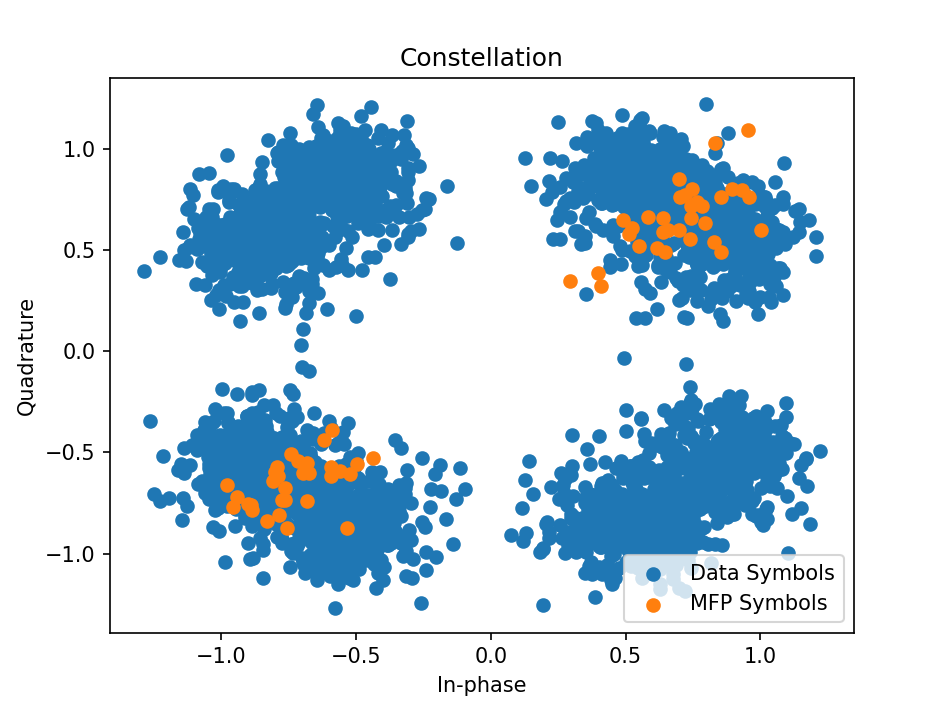
\includegraphics[width=0.5\textwidth]{mfp_constellation.png}}}
%	\caption{Constellation of MFP Symbols vs Data Symbols}
%	\label{fig::mfp_constellation}
%\end{figure}

%Examining the constellation, we see that the MFP is also bi-phase. To improve our correlation performance going forward, we demodulate each of the MFP constellation points. Note that our results are ambiguous by $180^{\circ}$ as described above. For now we assume a leading 1 in the MFPs.

% Add plot of FSP in constellation w/ different color

% Add picture of setup

\subsection{Convolutional Decoder}

In this section, we examine the Viterbi decoder output for a frame counter in the TSCC. With a single satellite, one can use either the top portion of the Viterbi decoder or the bottom portion depending on the chosen satellite.  With both satellites, the Viterbi is run at a rate 1/3 code rate.  When using a single satellite, the Viterbi decoder operates at an effective code rate of 1/2 with correct puncturing. This corresponds to a 3/4 encoder rate -- meaning that for every 4 received bits, 3 are usable as information bits.  The decoder however, consistently needs more than 3 transmission bits in order to determine the state of the trellis.

\begin{figure}[H]
	\centerline{\fbox{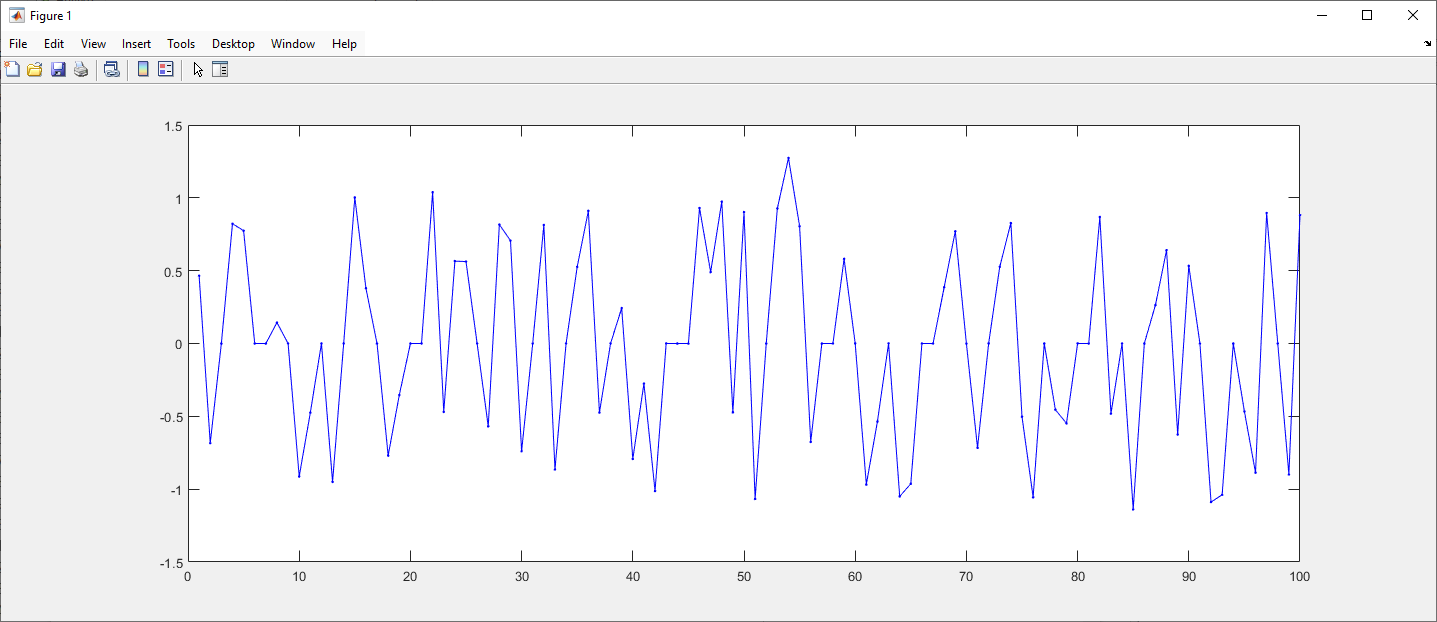
\includegraphics[width=0.8\textwidth]{Viterbi_insufficient_bits.png}}}
	\caption{XM Insufficient Data into Decoder}
	\label{fig::Viterbi_1}
\end{figure}

In Figure \ref{fig::Viterbi_1}, there is an insuffient number of input bits to a Viterbi decoder as the time interleaver is not completely full.  Since we are only using 1 satellite, the FEC is not capable of decoding this PRC block.  In Figure \ref{fig::Viterbi_2}, which is later in time, there is sufficient transmitted bits to use in the Viterbi decoder.

\begin{figure}[H]
	\centerline{\fbox{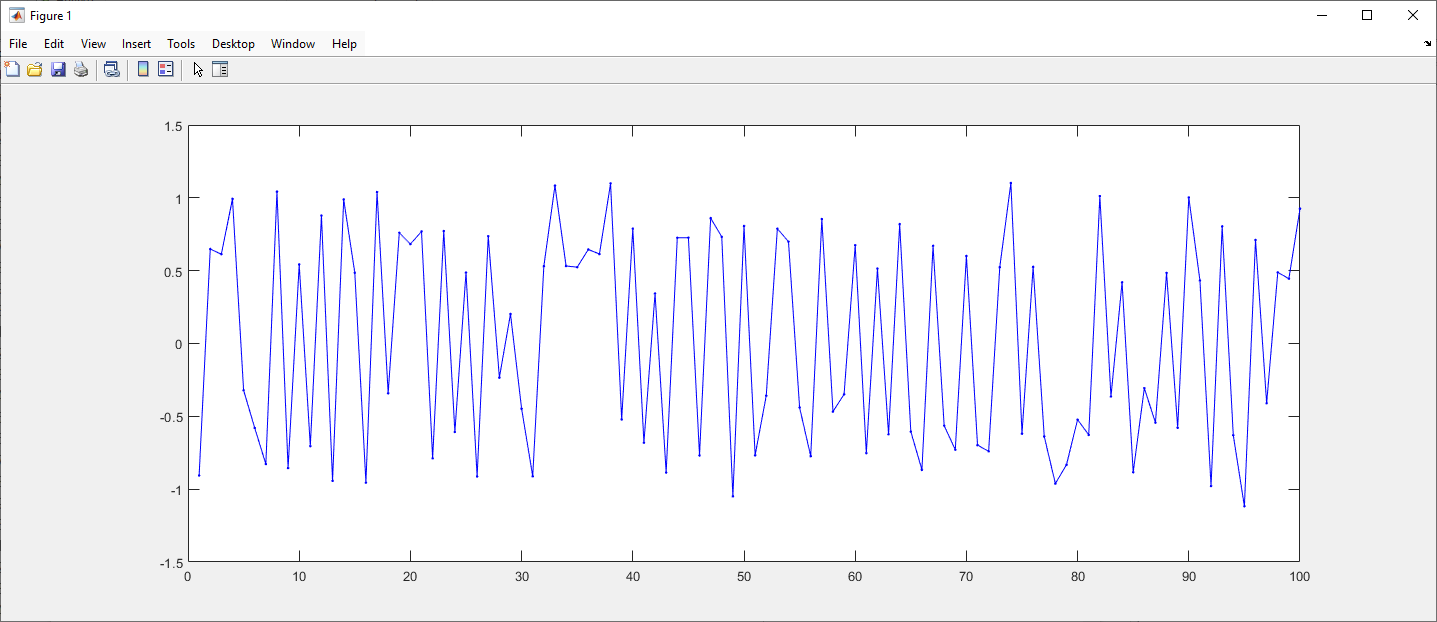
\includegraphics[width=0.8\textwidth]{Viterbi_sufficient_bits.png}}}
	\caption{XM Sufficient Data into Decoder}
	\label{fig::Viterbi_2}
\end{figure}

Over portions of the frame with sufficient data, we looked at the Viterbi output for satellite 2.  This was done using a MATLAB SPY plot.  As can be seen in Figure \ref{fig::Viterbi_spy}, the output does not show any structure in the vertical domain.  A frame counter was expected and not found.

\begin{figure}[H]
	\centerline{\fbox{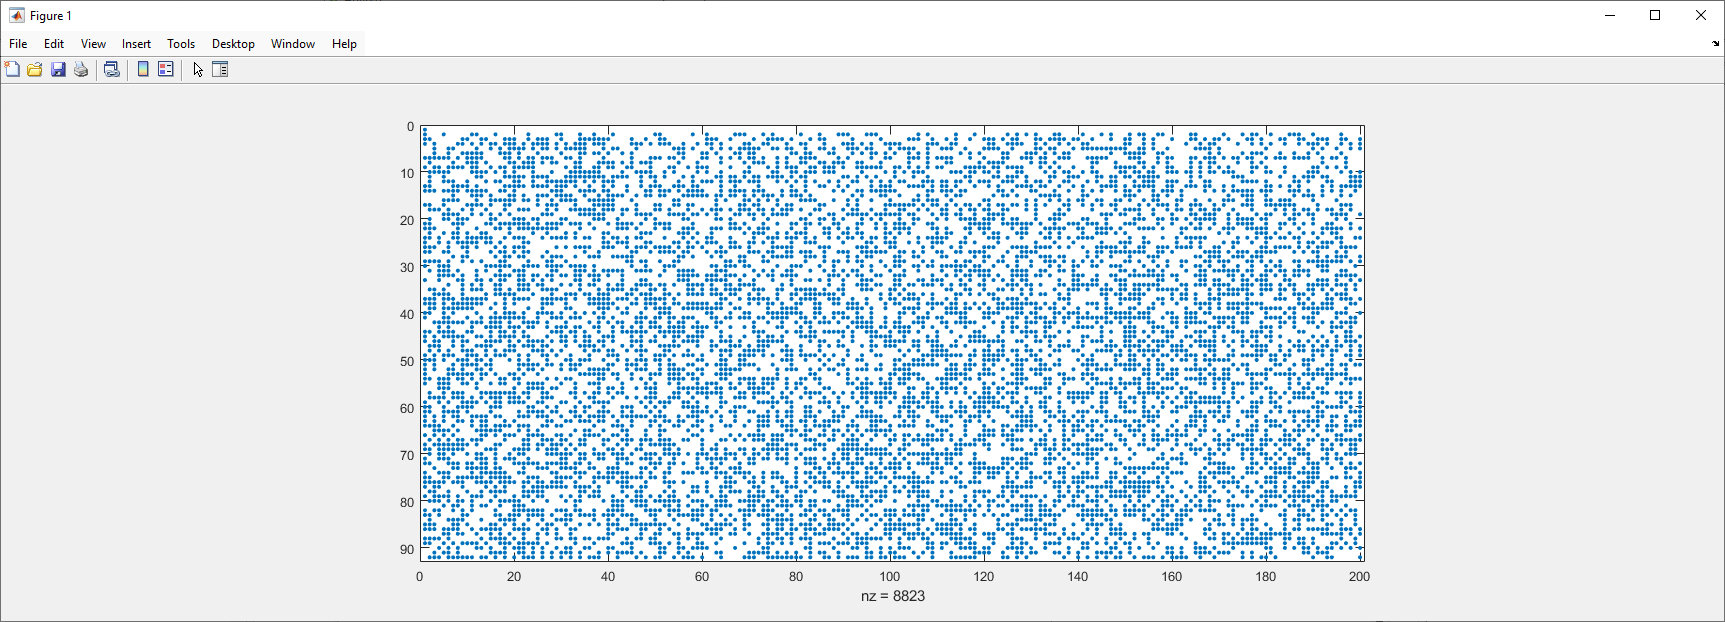
\includegraphics[width=0.8\textwidth]{Viterbi_SPY.png}}}
	\caption{XM Viterbi SPY output}
	\label{fig::Viterbi_spy}
\end{figure}

At this point we re-examined the documentation and discovered that the STA400a chipset showed a potential scrambler.  This was not included in any patent descriptions, nor was there any mention in the STA400a document of the scrambler implementation.  Resolving this unknown scrambler was outside the scope of our project.  A scrambler is sometimes used in digital communication systems to disperse energy so the timing and carrier recovery algorithms have transitions in the received symbols.  These are typically done with Linear Feedback Shift Registers (LFSR) and create a pseudo random sequence that is added to the original codeword in GF(2) space prior to transmission.  By applying the same pseudo random sequence at the receiver, the scrambling is removed.  This would be done between the timing/carrier recovery algorithm and FEC algorithm.

The absence of a descrambler would explain why no recognizable frame structure was observed in the Viterbi output, despite correct decoding procedures.  There was also mention of a RS block interleaver that was also undocumented except overview descriptions in the STA400a chipset.  Resolving the descrambler is required prior to resolving the block interleaver algorithm. 

\begin{figure}[H]
	\centerline{\fbox{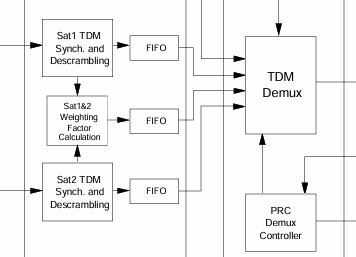
\includegraphics[width=0.8\textwidth]{XM_scrambler.png}}}
	\caption{XM Potential Scrambler \cite{alldatasheetcom_2015_sta400a}}
	\label{fig::scrambler}
\end{figure}

\subsection{Reed Solomon Decoding}

Because the Viterbi decoder output did not show the frame counter, we used only MATLAB generated data in our Reed Solomon decoder. In MATLAB, we specifically generated a free running counter output which wrapped into the range [0, 255].

\begin{figure}[H]
	\centerline{\fbox{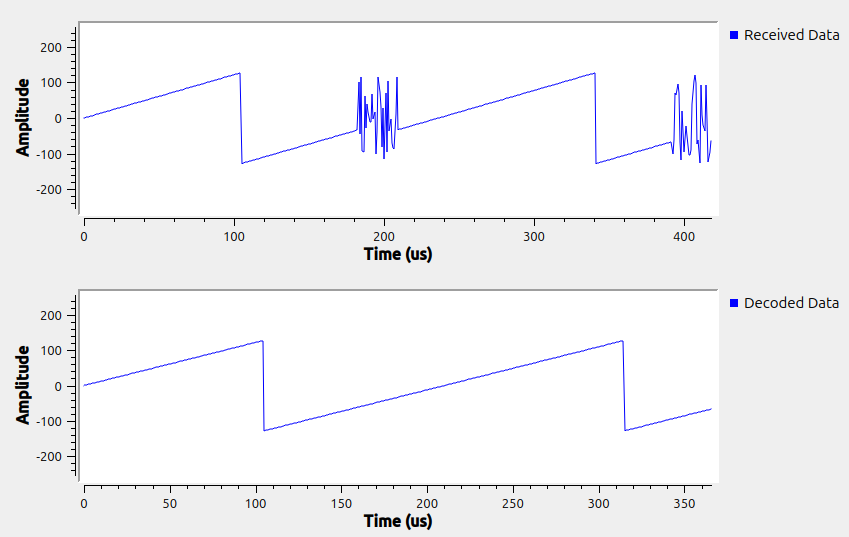
\includegraphics[width=0.8\textwidth]{RS_decoder_output.png}}}
	\caption{RS Decoder Input and Output for a Free-Running Counter}
	\label{fig::RS_decoder_output}
\end{figure}

In the input data, we observed our transmitted message and parity bits (noisy spikes). Because there were no errors in our transmitted message, the Reed Solomon decoder output was simply the first 223 bytes in the received data. We also experimented with the error correction capabilities of the RS decoder by inserting random errors into our input data. The inputs and outputs with the additional errors are illustrated below in Figure \ref{fig::RS_decoder_output_errors}.

\begin{figure}[H]
	\centerline{\fbox{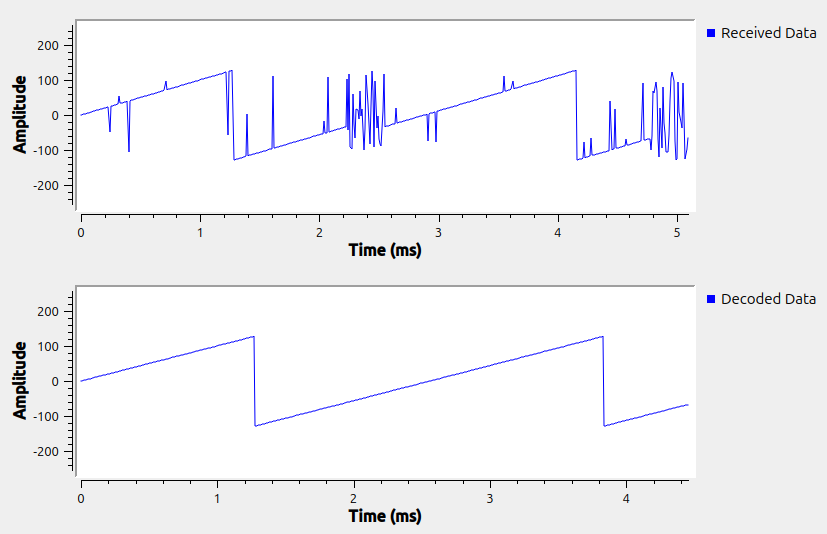
\includegraphics[width=0.8\textwidth]{RS_decoder_output_errors.png}}}
	\caption{RS Decoder Input and Output Demonstrating Error Correction}
	\label{fig::RS_decoder_output_errors}
\end{figure}

Examining the input data, we see that it has byte errors in addition to the preamble. However, after running the Reed Solomon decoder, we have shown that we can correct for each of these errors. While not fully integrated with the XM radio chain, our Reed Solomon decoder can easily be added once the descrambler is in place.

%In this section, we experiment with

\iffalse
\begin{itemize}
	\item Nyquist Filter
	\item Timing Synchronization
	\item Carrier Compensation
	\begin{itemize}
		\item Coarse
		\item Fine
	\end{itemize}
	\item Frame Synchronization
\end{itemize}
\fi

\printbibliography

\iffalse
\nocite{5586866}
\nocite{a2008_us8260192b2}
\nocite{marko_2012_us8667344b2}
\nocite{collins_2018_softwaredefined}
\nocite{chaudhari_2022_timing}
\nocite{650240}
\bibliographystyle{IEEEtran}
\bibliography{sources}{}
%\bibliographystyle{ieeetr}
\fi
\end{document}